\documentclass[hyperref=colorlinks]{beamer}
\mode<presentation>
\usetheme{iclpt}
\setbeamertemplate{navigation symbols}{}
\setbeamertemplate{headline}{
  \begin{beamercolorbox}[leftskip=.2cm,rightskip=.2cm,topskip=.2cm,ht=1.1cm,dp=0.1cm,wd=\textwidth]{institute in head/foot}
    
\includegraphics[height=1cm]{icl.pdf}
    \hfill
    \includegraphics[height=1cm]{../Pics/ATLAS-Logo-Square-Blue-RGB.png}
    
\includegraphics[height=1cm]{../Pics/CMS-Color.pdf}
  \end{beamercolorbox}
}
\setbeamertemplate{footline}{
  \begin{beamercolorbox}[ht=.35cm,dp=0.2cm,wd=\textwidth,leftskip=.3cm]{author in head/foot}%
    \begin{minipage}[c]{5cm}%
      \usebeamerfont{author in head/foot}
      \insertshortauthor 
      \insertshorttitle
    \end{minipage}\hfill%
    \hfill
    \insertframenumber{} / \ref{lastframe}
    %\hfill
    \begin{minipage}{6cm}
      \hfill
      %\insertshorttitle
    \end{minipage}
  \end{beamercolorbox}%
}

\definecolor{beamer@icdarkblue}{RGB}{0,51,102}
\definecolor{beamer@icmiddleblue}{RGB}{0,82,150} 
\definecolor{beamer@iclightblue}{RGB}{200,212,232}
\definecolor{beamer@icmiddlered}{RGB}{204,51,0}
\definecolor{beamer@iclightred}{RGB}{232,212,32}

\usepackage{tikz}
\usetikzlibrary{arrows,shapes,backgrounds}
\usepackage{color}
\usepackage{tabularx,colortbl}
\usepackage{graphicx}
\usepackage{pdfpages}
\usepackage{feynmp}
\usepackage{rotating}
\usepackage{moresize}
\usepackage{slashed}
\usepackage{xcolor,colortbl}
\DeclareGraphicsRule{*}{mps}{*}{}
\hypersetup{colorlinks=false}

\title[Latest results on invisibly decaying Higgs bosons]{\vspace{-0.2cm} Latest results on invisibly decaying Higgs bosons}
\author[P. Dunne]{Patrick Dunne - Imperial College London \\ on behalf of the ATLAS and CMS Collaborations \\ DM@LHC 2016 - 31/03/2016}
\titlegraphic{
  \vspace{-0.4cm}
  \begin{fmffile}{dmlhcfeyndiagstitle}
    \begin{fmfgraph*}(75,75)
      \fmfleft{i0,i2,ix,i3,i5}
      \fmfright{o0,o3,o1,o4,o6}
      \fmf{phantom,tension=4/3}{i2,v1,o3}
      \fmf{phantom,tension=4/3}{i3,v2,o4}
      \fmffreeze
      \fmf{gluon,tension=4/3}{i2,v1}
      \fmf{gluon,tension=4/3}{i3,v2}
      \fmf{fermion,tension=0}{v1,v2}
      \fmf{fermion,tension=2/3}{v2,v3,v1}
      \fmf{dashes}{v3,o1}
      \fmflabel{$g$}{i2}
      \fmflabel{$g$}{i3}
      \fmflabel{$H$}{o1}
    \end{fmfgraph*}    
    \hspace{.5cm}
    \begin{fmfgraph*}(75,75)
      \fmfleft{i1,i2}
      \fmfright{o1,o2,o3}
      \fmf{fermion}{i1,v1,o1}
      \fmf{fermion}{i2,v2,o3}
      \fmf{photon,label=$W,,Z$}{v1,v3}
      \fmf{photon,label=$W,,Z$}{v2,v3}
      \fmf{dashes}{v3,o2}
      \fmflabel{$q$}{i1}
      \fmflabel{$q$}{i2}
      \fmflabel{$q$}{o1}
      \fmflabel{$q$}{o3}
      \fmflabel{$H$}{o2}
    \end{fmfgraph*}
    \hspace{.5cm}
    \begin{fmfgraph*}(75,75)
      \fmfleft{i1,i2}
      \fmfright{o1,o2}
      \fmf{fermion}{i1,v1}
      \fmf{fermion}{v1,i2}
      \fmf{photon,label=$W,,Z$}{v1,v2}
      \fmf{photon}{v2,o1}
      \fmf{dashes}{v2,o2}
      \fmflabel{$q$}{i1}
      \fmflabel{$\bar{q}$}{i2}
      \fmflabel{$W,Z$}{o1}
      \fmflabel{$H$}{o2}
    \end{fmfgraph*}
  \end{fmffile}
  %% \begin{fmfgraph*}(100,70)
  %%         \fmfleft{i1,i2}
  %%         \fmfright{o1,o2,o3}
  %%         \fmf{fermion}{i1,v1,o1}
  %%         \fmf{fermion}{i2,v2,o3}
  %%         \fmf{phantom,tension=4/5}{v1,v2}
  %%         \fmffreeze
  %%         \fmf{photon,label=$W,,Z$}{v1,v3}
  %%         \fmf{photon,label=$W,,Z$}{v2,v3}
  %%         \fmf{dashes}{v3,o2}
  %%         \fmflabel{$q$}{i1}
  %%         \fmflabel{$q$}{i2}
  %%         \fmflabel{$q$}{o1}
  %%         \fmflabel{$q$}{o3}
  %%         \fmflabel{$H$}{o2}

  %%       \end{fmfgraph*}
}
\date{}
\begin{document}
\tikzstyle{every picture}+=[remember picture]
\tikzstyle{na} = [baseline=-.5ex]
\begin{fmffile}{dmlhcfeyndiags}


  %TITLE PAGE
  %20 mins + 5 questions
  \section{Title}
  \begin{frame}
    \titlepage
  \end{frame}

  \begin{frame}
    \frametitle{Outline}
    \begin{block}{}
      \begin{itemize}
      \item How to search for invisibly decaying Higgs bosons:
      \item[-] direct and indirect searches
      \item Run 1 results from ATLAS and CMS
      \item Run 2 results from CMS
      \item Projections of future sensitivity
      \item nb all limits at 95\% CL unless stated otherwise
      \end{itemize}
    \end{block}
  \end{frame}

  \begin{frame}
    \frametitle{Why look for invisibly decaying Higgs bosons?}
    \vspace{-.3cm}
    \begin{columns}
      \column{1.06\textwidth}
    \begin{block}{Theoretical Motivations}
      \small
      \begin{itemize}
      \item All SM massive particles get their mass through Higgs boson couplings
      \item Why not dark matter?
      \end{itemize}
    \end{block}
    \end{columns}

    \vspace{-.2cm}    

    \begin{columns}
    \column{.55\textwidth}
    \begin{block}{Experimental motivation}
      \small
      \begin{itemize}
      \item Measurements of the Higgs boson made so far are impressive:
        \vspace{-.1cm}
      \item[-] Mass measured with 0.2\% error
      \item A lot of parameters are still relatively unconstrained:
        \vspace{-.1cm}
      \item[-] Limit on width is $\sim$4$\Gamma_{SM}$
      \item Plenty of room for Higgs boson couplings to dark matter
      \end{itemize}
    \end{block}
    \column{.45\textwidth}
    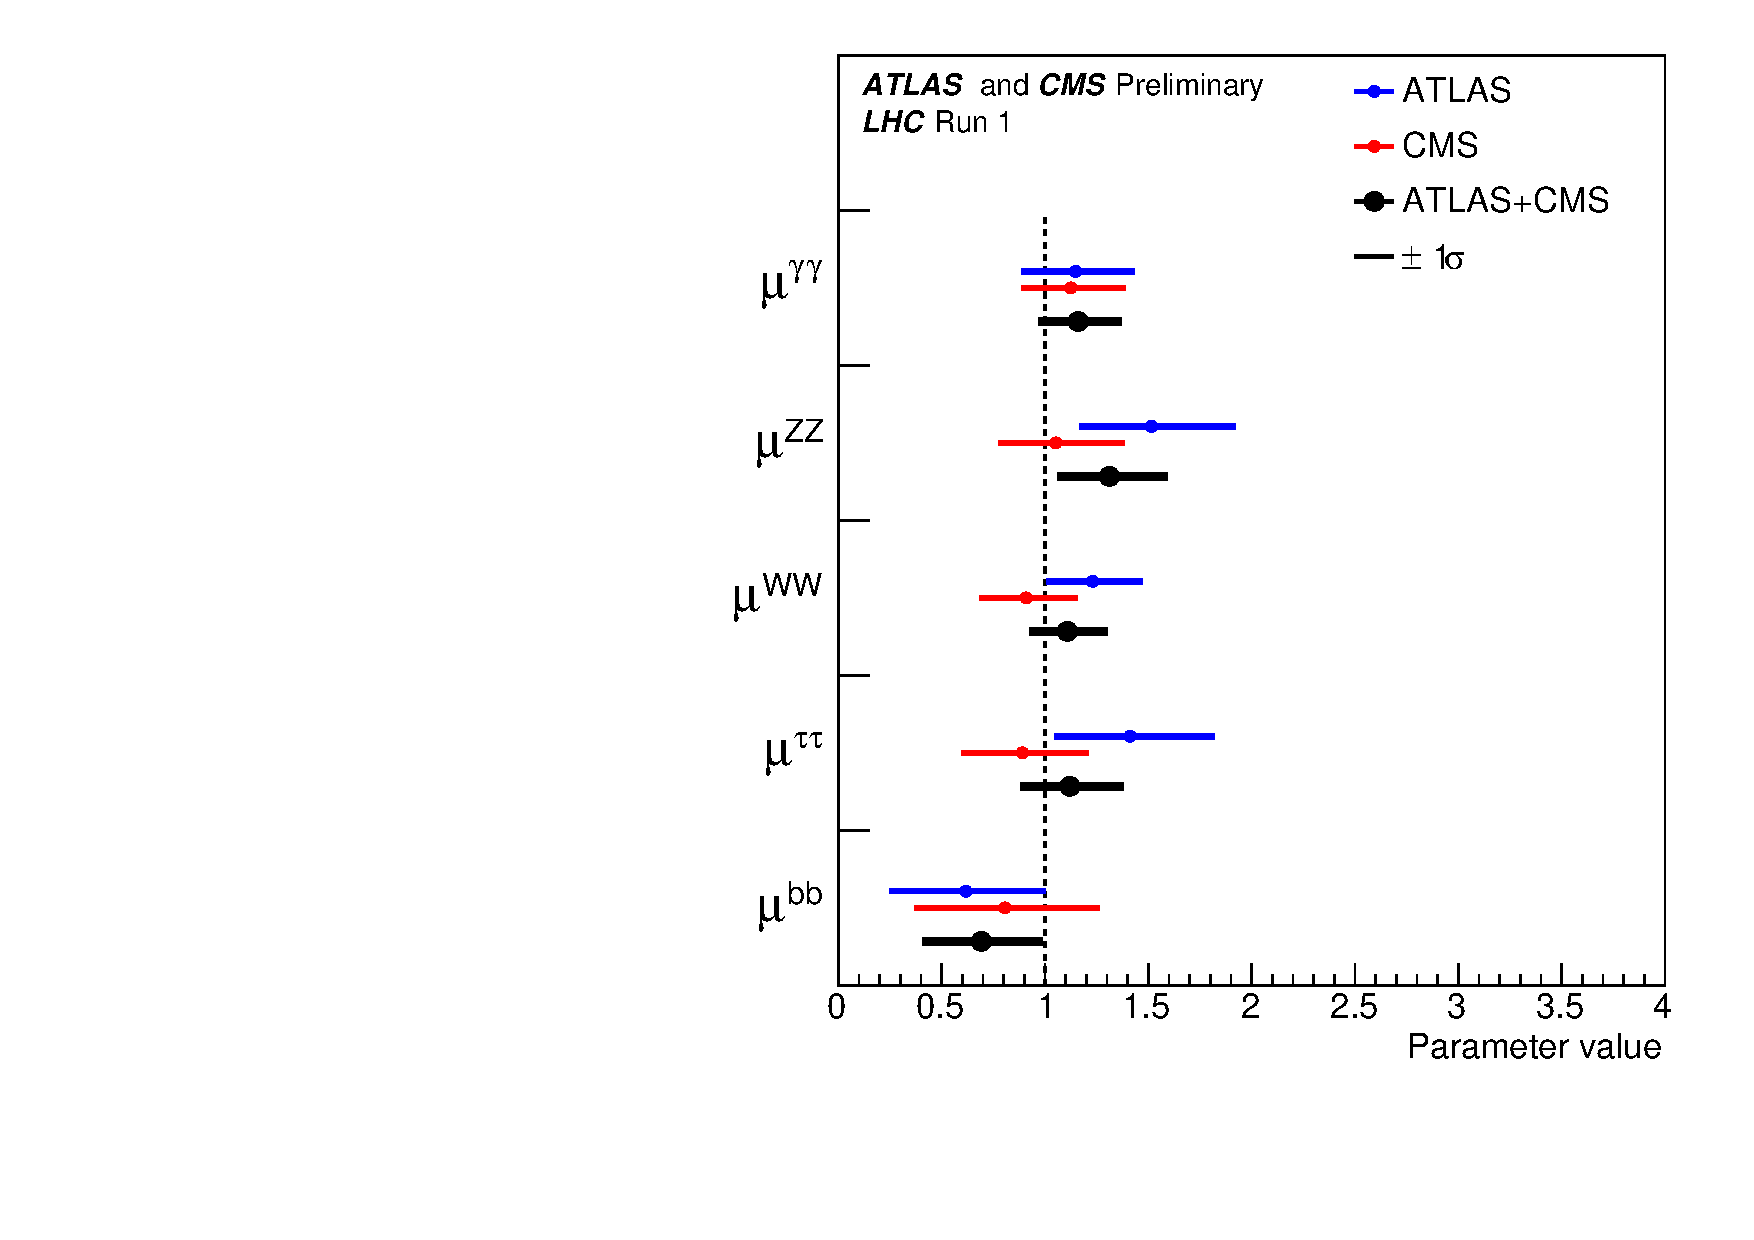
\includegraphics[width=\textwidth]{TalkPics/DM@LHC2016/CMS-PAS-HIG-15-002_Figure_012.pdf}
      \centering
      \scriptsize

      CMS-PAS-HIG-15-002
      
      ATLAS-CONF-2015-044
    \end{columns}
  \end{frame}

  \begin{frame}
    \frametitle{How to search for invisibly decaying Higgs bosons}
    \vspace{-.2cm}
    \begin{columns}
      \column{.5\textwidth}
      \begin{block}{Indirect searches}
          \small
          \begin{itemize}
          \item Compare visible width to total width:
          \item[-] $\rm{BR}_{BSM}=\frac{\Gamma_{H}-\Gamma_{vis}}{\Gamma_{H}}$
          \item No measurement of $\Gamma_{H}$, need to make an assumption
          \item[-] Usually assume SM width
          \item ATLAS+CMS combination gives an observed (expected) limit on $\rm{BR}_{BSM}$ of 0.34 (0.35)
          \end{itemize}
      \end{block}
      \column{.5\textwidth}
      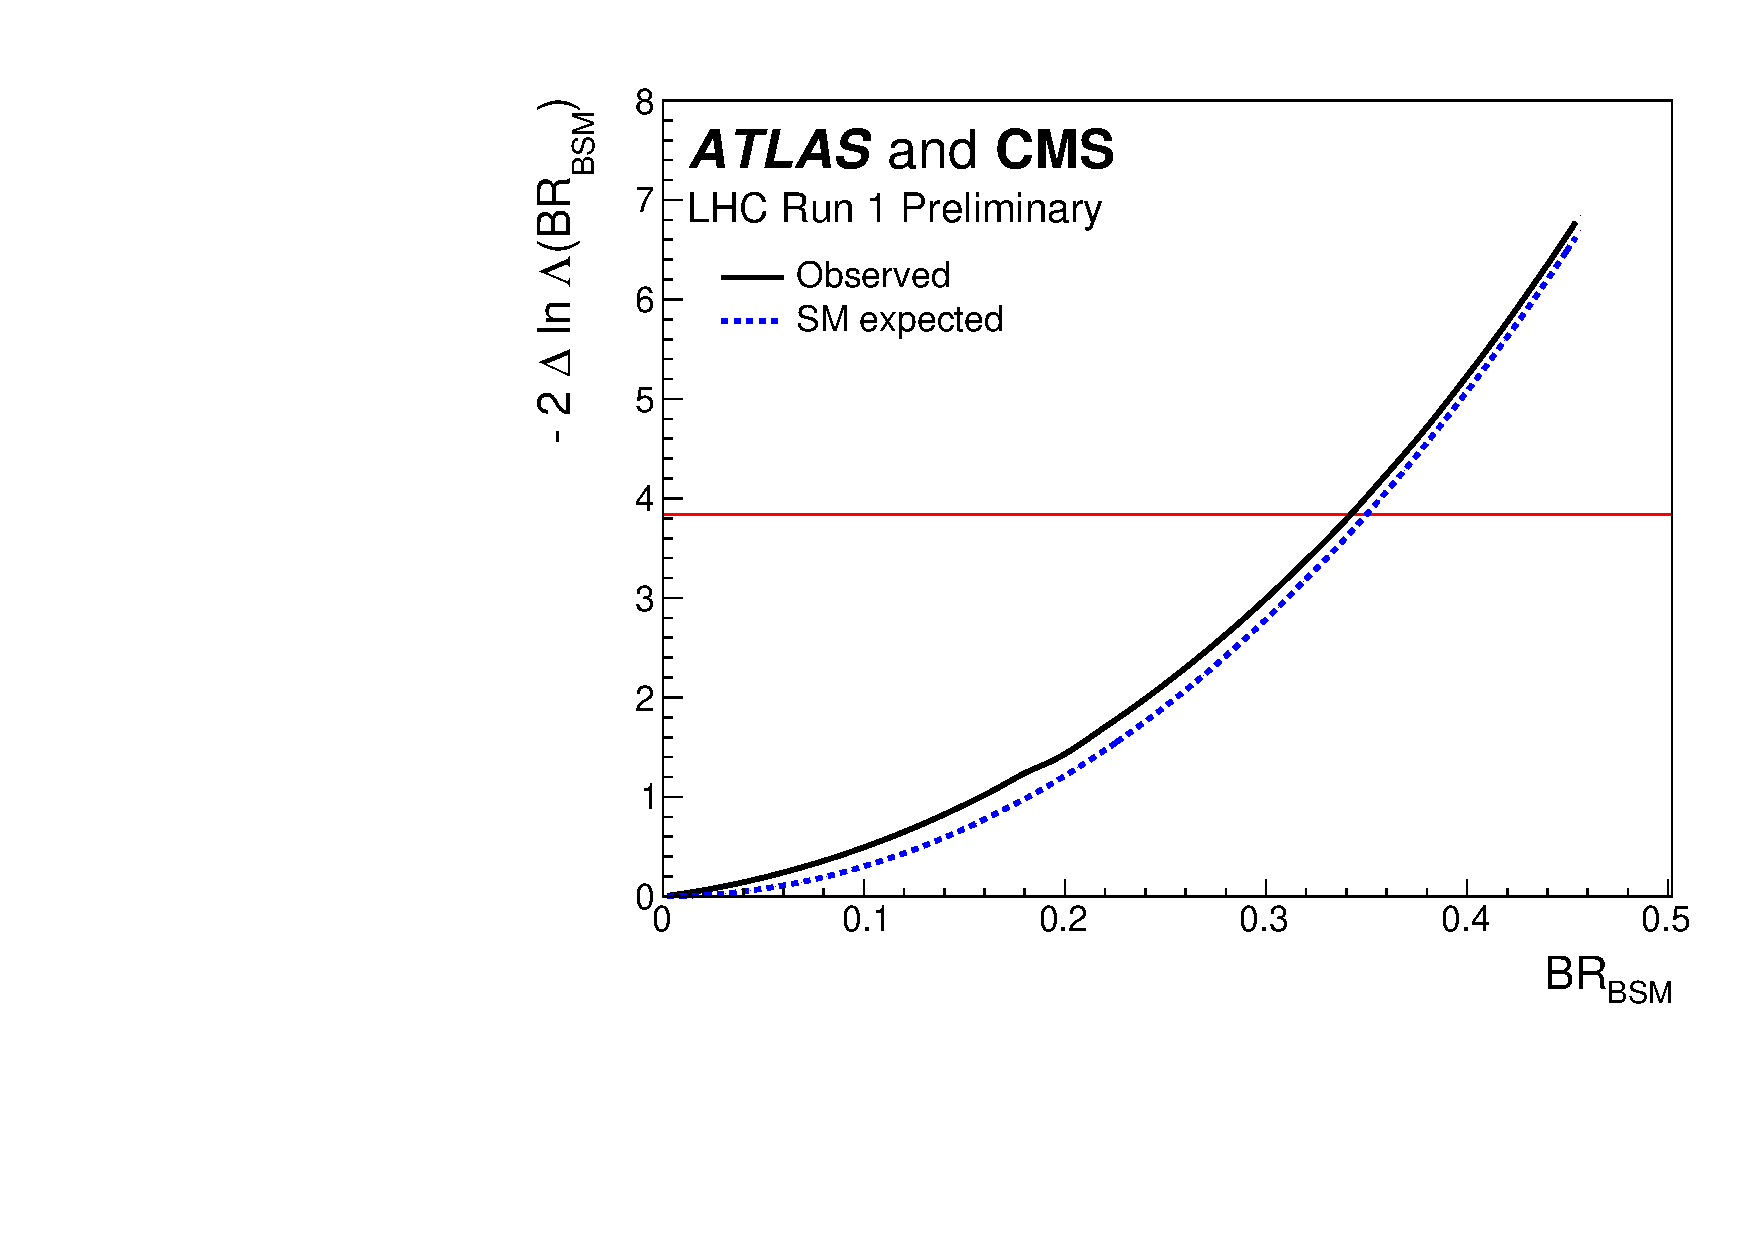
\includegraphics[width=\textwidth]{TalkPics/DM@LHC2016/CMS-PAS-HIG-15-002_Figure_015.pdf}
      \centering
      \scriptsize

      CMS-PAS-HIG-15-002
      
      ATLAS-CONF-2015-044
       \end{columns}
       %ATLAS or CMS rates of each channel plot
  \end{frame}

  \begin{frame}
    \frametitle{How to search for invisibly decaying Higgs bosons}
    \begin{columns}
      \column{1.06\textwidth}
    \begin{block}{}
      \small
      \begin{itemize}
      \item Look for associated Higgs boson products plus $E_{T}^{miss}$
      \end{itemize}
    \end{block}
    \end{columns}
    \begin{columns}
      \column{.5\textwidth}
      \begin{block}{Production channels}
          \small
          %??ggH, VBF, VH tikz lines to plot if time
          \begin{itemize}
          \item VBF mode is most sensitive
          \item[-] Second highest rate and distinctive topology
          \item Gluon fusion has no visible products, needs ISR
          \item[-] High rate, difficult final state
          \item VH has clean final states but low rate
          \end{itemize}
      \end{block}
      \column{.5\textwidth}
      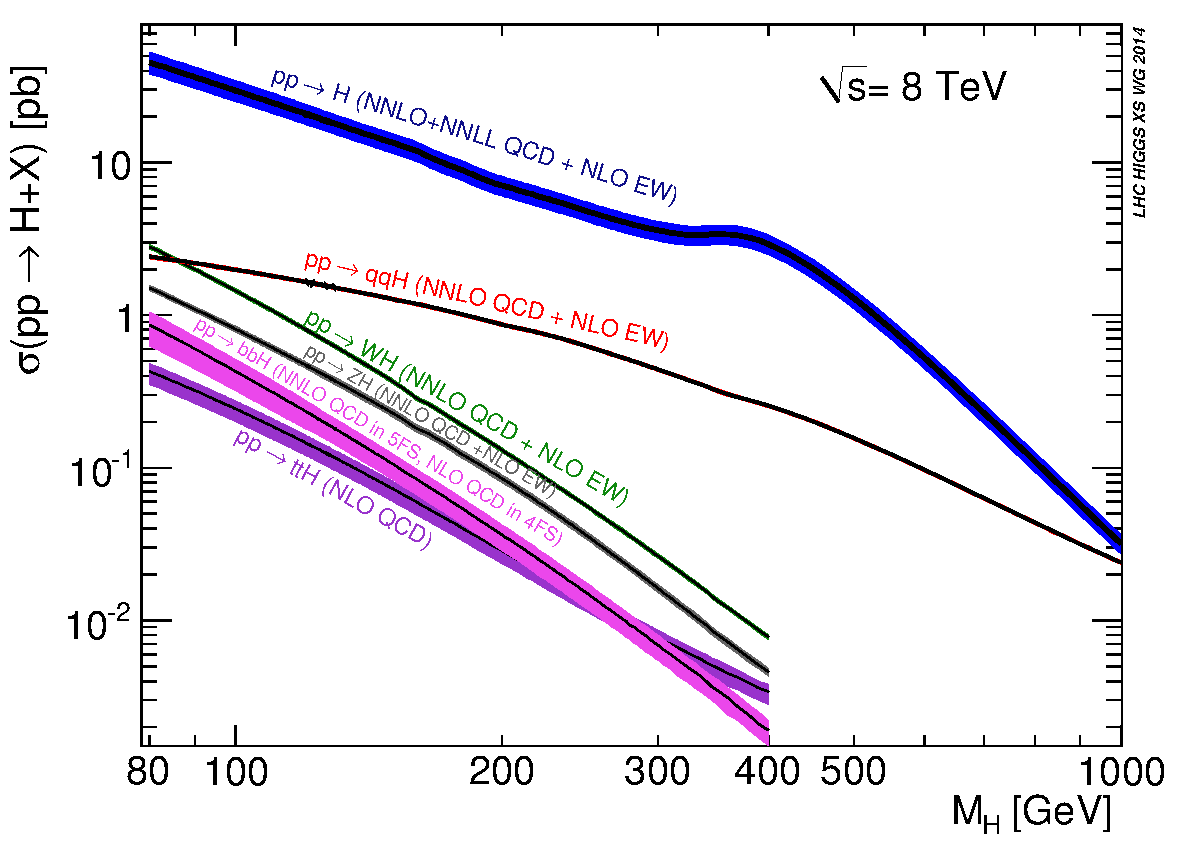
\includegraphics[width=\textwidth]{TalkPics/DM@LHC2016/XS_8TeV-eps-converted-to.pdf}
      \end{columns}
    \end{frame}

  %??ATLAS RUN 1 
  \begin{frame}
    %ZH http://journals.aps.org/prl/abstract/10.1103/PhysRevLett.112.201802
    \frametitle{Run 1 ATLAS direct searches - Z($\ell\ell$)H}
    %search description and limit
    \begin{columns}
      \column{.5\textwidth}
      \begin{block}{}
        \small
        \begin{itemize}
        \item Selects two leptons opposite large $E_{T}^{miss}$
        \item $E_{T}^{miss}$ Shape analysis with data driven backgrounds
        \item Observed (expected) limit on $\mathcal{B}\left(H\rightarrow inv.\right)$ for $m_{H}=$125.5 GeV is 75 (62)\%
        \end{itemize}
      \end{block}
      \column{.5\textwidth}
      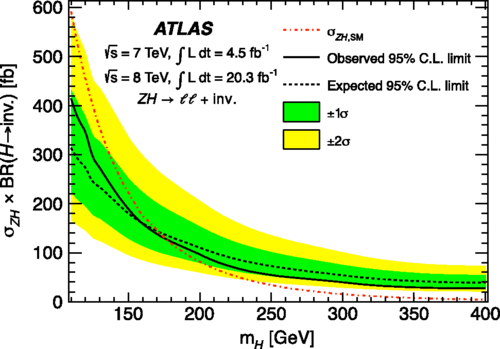
\includegraphics[width=\textwidth]{TalkPics/DM@LHC2016/ATLASZH.png}
      \centering
      \scriptsize
      
      PRL 112, 201802 (2014)
    \end{columns}
  \end{frame}

  \begin{frame}
    %V(had)H: http://arxiv.org/abs/1504.04324
    \frametitle{Run 1 ATLAS direct searches - V(had)H}
    %search description and limit
    \begin{columns}
      \column{.5\textwidth}
      \begin{block}{}
        \small
        \begin{itemize}
        \item Targets $W/Z\rightarrow qq$ final state
        \item $E_{T}^{miss}$ and dijet $p_{T}$ shape analysis with data driven backgrounds
        \item Observed (expected) limit on $\mathcal{B}\left(H\rightarrow inv.\right)$ for $m_{H}=$125 GeV is 78 (86)\%
        \end{itemize}
      \end{block}
      \column{.5\textwidth}
      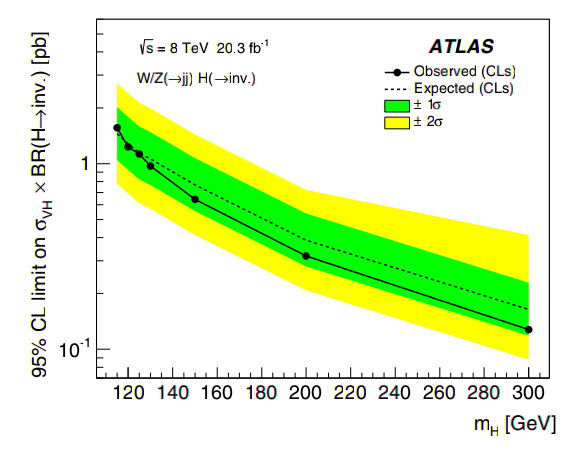
\includegraphics[width=\textwidth]{TalkPics/DM@LHC2016/ATLASVH.png}
      \centering
      \scriptsize

      Eur. Phys. J. C (2015) 75:337
    \end{columns}
  \end{frame}

  \begin{frame}
    %http://arxiv.org/pdf/1508.07869v2.pdf
    \frametitle{Run 1 ATLAS direct searches - VBF}
    %search description and limit mention tying W and Z together
    \begin{columns}
      \column{.5\textwidth}
      \begin{block}{}
        \small
        \begin{itemize}
        \item Select two jets with large $\Delta\eta$ opposite large $E_{T}^{miss}$
        \item Counting experiment with data driven background estimation
        \item[- ] $W\rightarrow e\nu$, $W\rightarrow \mu\nu$ and $W\rightarrow \tau\nu$ and $Z\rightarrow \nu\nu$ normalisation tied together
        \item Observed (expected) limit on $\mathcal{B}\left(H\rightarrow inv.\right)$ for $m_{H}=$125 GeV is 28 (31)\%
        \end{itemize}
      \end{block}
      \column{.5\textwidth}
      %??no mas scan find another pic to use
      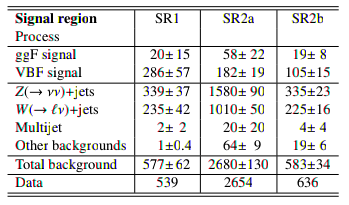
\includegraphics[width=\textwidth]{TalkPics/DM@LHC2016/ATLASvbfyields.png}
      \centering
      \scriptsize

      JHEP 01 (2016) 172
    \end{columns}
  \end{frame}

  \begin{frame}
    %http://arxiv.org/pdf/1509.00672v2.pdf (fig 8)
    %comb with vis
    \frametitle{Run 1 ATLAS direct searches - Combination}
    \begin{columns}
      \column{.5\textwidth}
      \begin{block}{}
        \small
        \begin{itemize}
        \item Combining searches significantly improves limits
        \item Direct searches provide most sensitivity
        \item[-] Observed (expected) limit on $\mathcal{B}\left(H\rightarrow inv.\right)$ for $m_{H}=$125 GeV is 25 (27)\%
        \item Adding indirect results adds assumption on Higgs total width 
        \item[-] Observed (expected) limit on $\mathcal{B}\left(H\rightarrow inv.\right)$ for $m_{H}=$125 GeV is 23 (24)\%
        \end{itemize}
      \end{block}
      \column{.5\textwidth}
      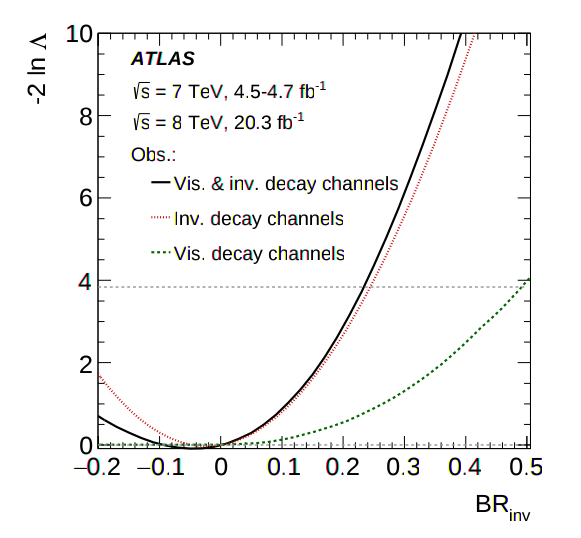
\includegraphics[width=\textwidth]{TalkPics/DM@LHC2016/ATLASviscomb.png}
      \centering
      \scriptsize

      JHEP11(2015)206
    \end{columns}
  \end{frame}



  %??CMS Run 1
  \begin{frame}
    %HIG-13-030
    \frametitle{Run 1 CMS direct searches - ZH}
    \begin{columns}
      %quick description comb from hig-13-030
      \column{.5\textwidth}
      \begin{block}{}
        \small
        \begin{itemize}
        \item Searches in $Z\rightarrow\ell\ell$ and $Z\rightarrow b\bar{b}$ channels
        \item $Z(\ell\ell)H$ search is a 2D shape analysis with data driven backgrounds
        \item $Z(b\bar{b})H$ search is a BDT shape analysis with data driven backgrounds
        \item Combined $ZH$ searches observed (expected) limit on $\mathcal{B}\left(H\rightarrow inv.\right)$ for $m_{H}=$125 GeV is 81 (83)\%
        \end{itemize}
      \end{block}
      \column{.5\textwidth}
      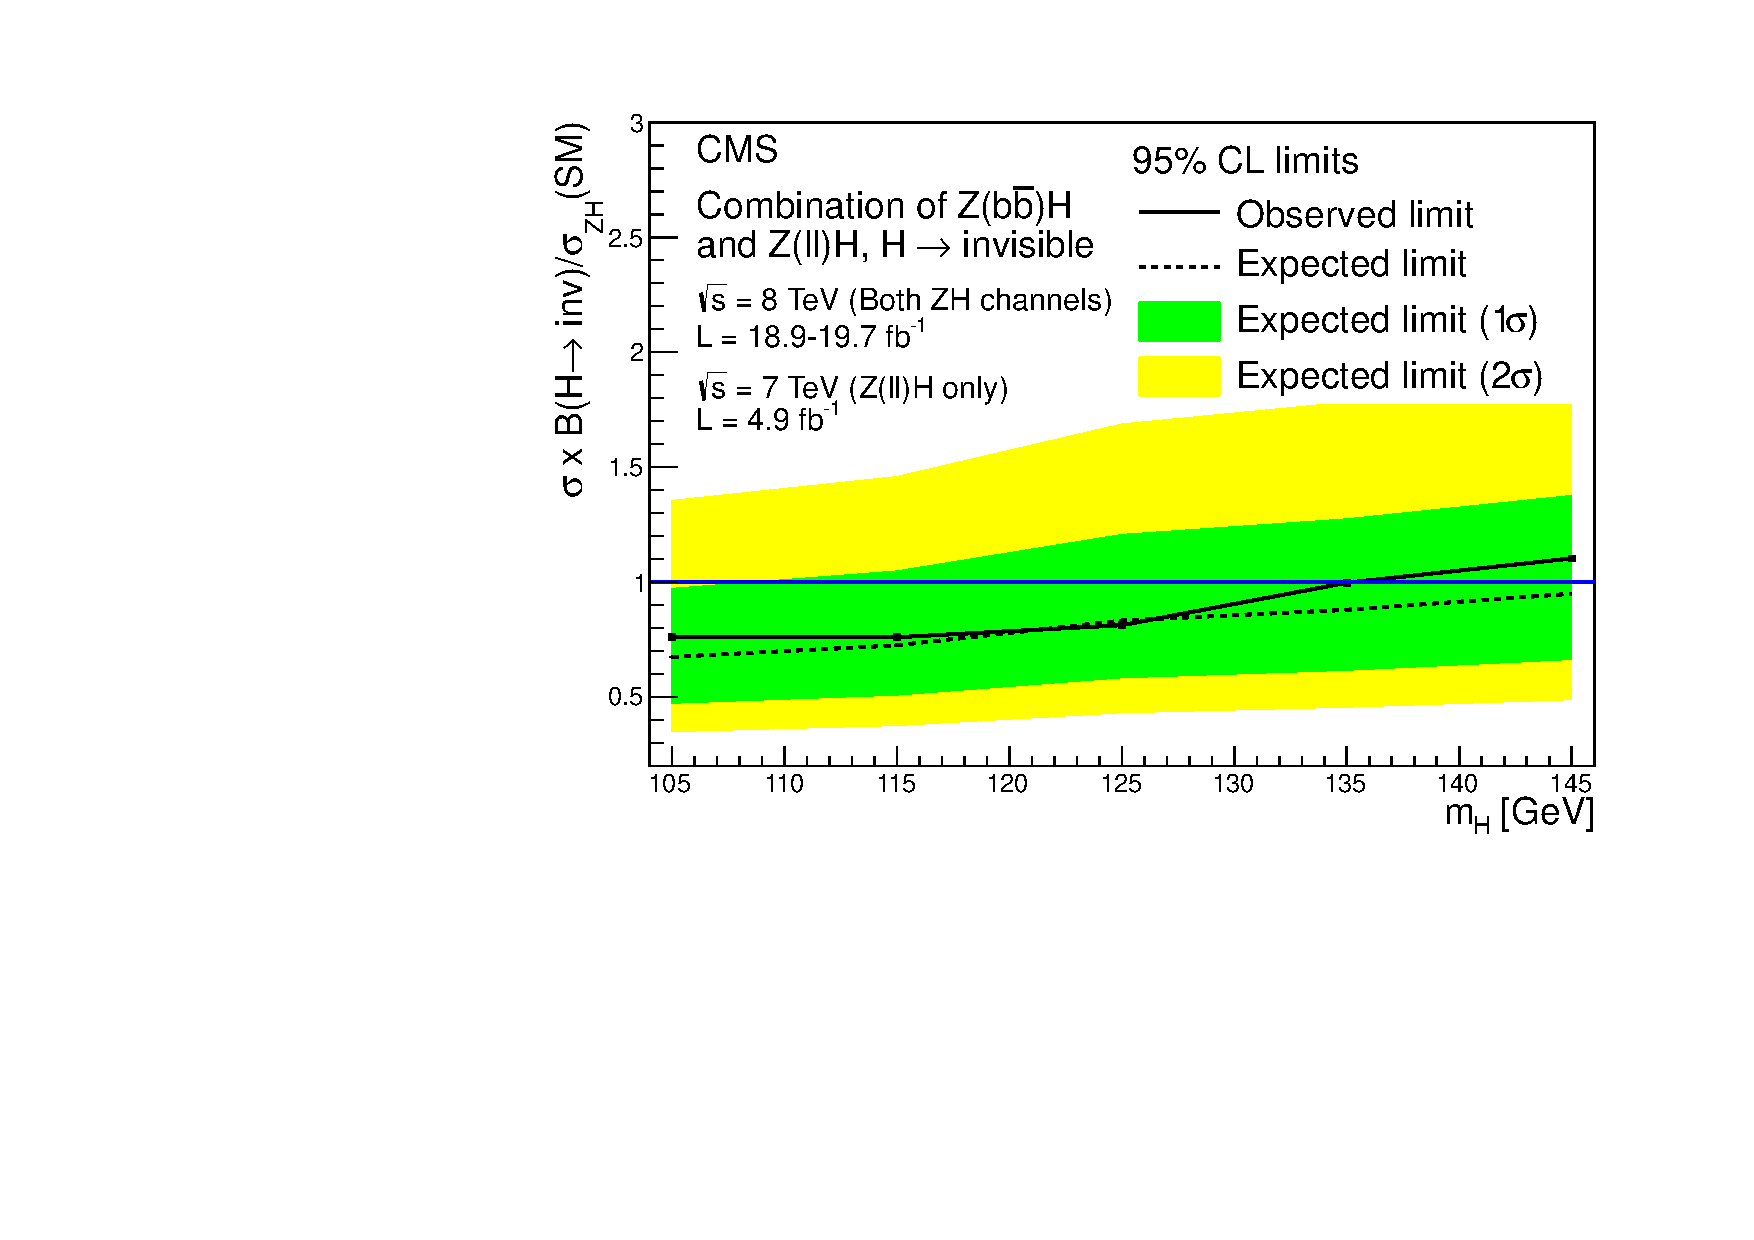
\includegraphics[width=\textwidth]{TalkPics/DM@LHC2016/Fig9b-ZH-LimitNorm.pdf}      
      \centering
      \scriptsize
      
      Eur. Phys. J. C 74 (2014) 2980
    \end{columns}
  \end{frame}

  \begin{frame}
    %??EXO-12-055
    \frametitle{Run 1 CMS direct searches - Monojet+V(had)H}
    \begin{columns}
      %??quick description
      \column{.5\textwidth}
      \begin{block}{}
        \small
        \begin{itemize}
        \item Search has categaries targeting $V(had)H$ and $ggH$ production modes
        \item $E_{T}^{miss}$ shape analysis with data driven background estimation
        \item Observed (expected) limit on $\mathcal{B}\left(H\rightarrow inv.\right)$ for $m_{H}=$125 GeV is 53 (62)\%
        \end{itemize}
      \end{block}
      \column{.5\textwidth}
      %??fig 8b from pas
      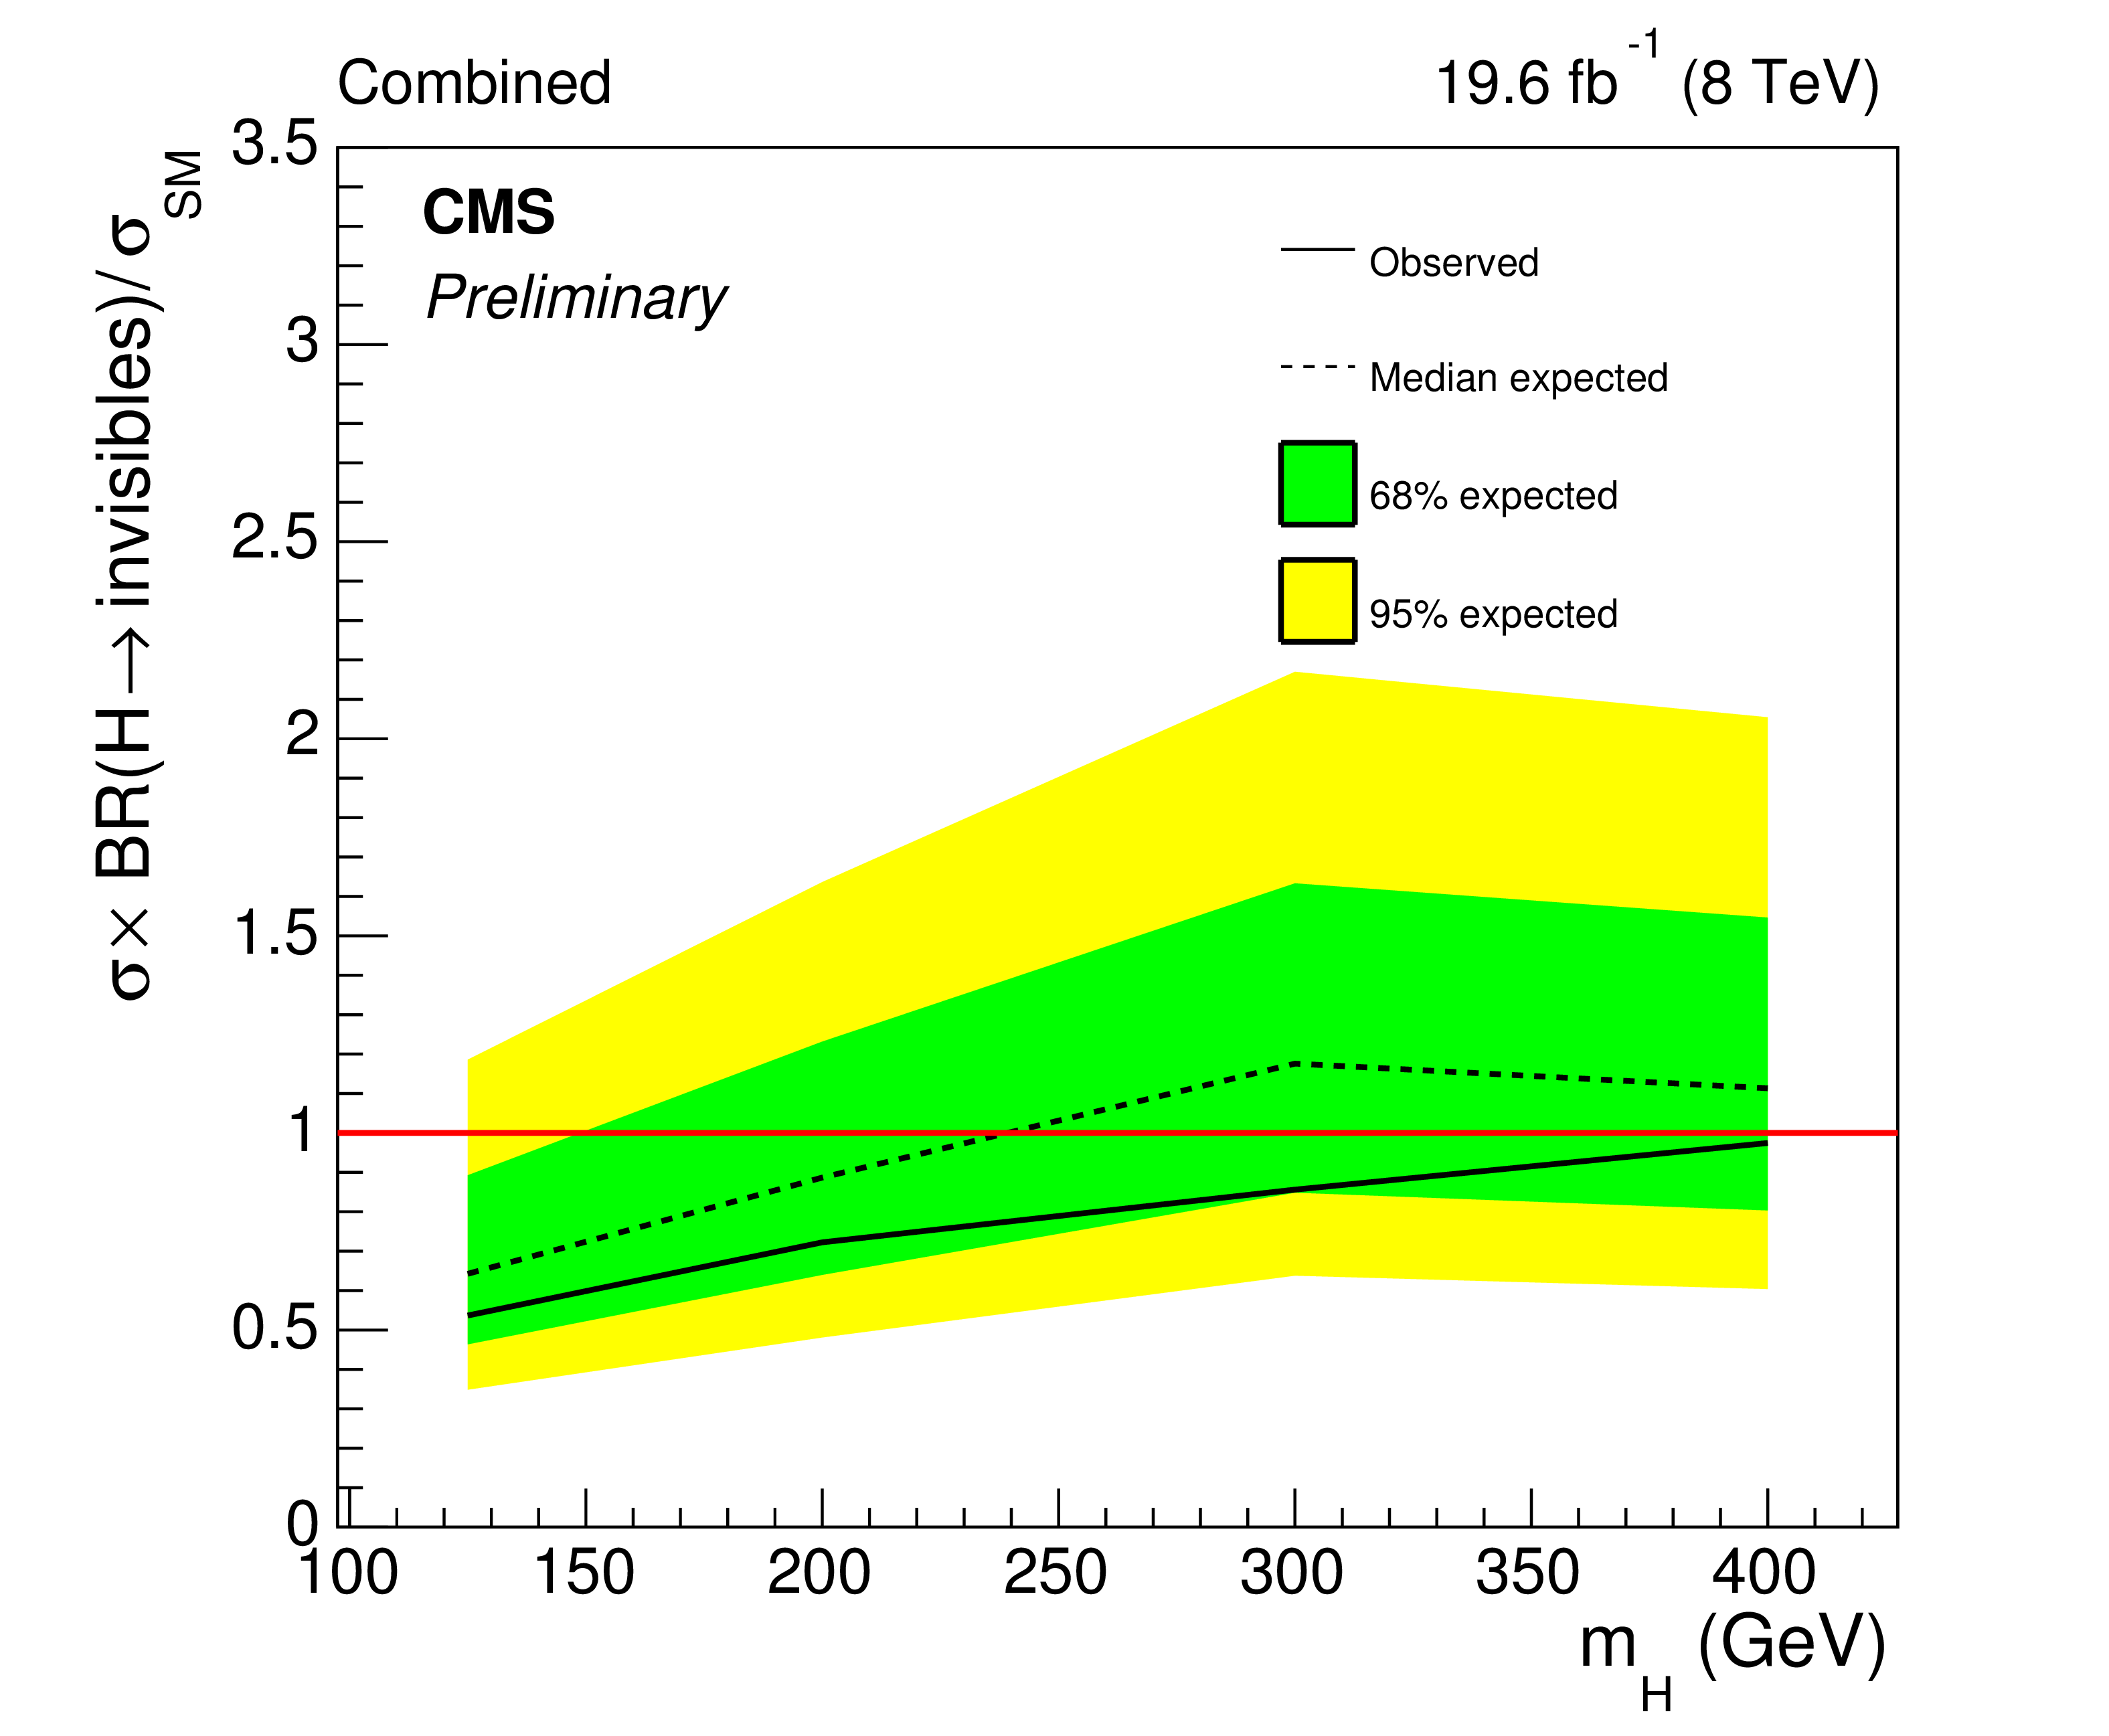
\includegraphics[width=\textwidth]{TalkPics/DM@LHC2016/CMS-PAS-EXO-12-055_Figure_008-b.png}
      \centering
      \scriptsize
      
      CMS-PAS-EXO-12-055
    \end{columns}
  \end{frame}

  \begin{frame}
    %??HIG-14-038
    \frametitle{Run 1 CMS direct searches - VBF}
    \begin{columns}
      %??quick description of parked data  
      \column{.5\textwidth}
      \begin{block}{}
        \small
        \begin{itemize}
        \item Select two jets with large $\Delta\eta$ separated from large $E_{T}^{miss}$
          \vspace{-.1cm}
        \item Dedicated ``parked data'' trigger
          \vspace{-.1cm}
        \item Counting experiment with data driven backgrounds
          \vspace{-.2cm}
        \item[-] V+jets backgrounds separately normalised
          \vspace{-.2cm}
        \item[-] If all normalisations had same uncertainty as $W\rightarrow\mu\nu$ expected limit would be 33\%
          \vspace{-.1cm}
        \item Observed (expected) limit on $\mathcal{B}\left(H\rightarrow inv.\right)$ for $m_{H}=$125 GeV is 57 (40)\%
        \end{itemize}
      \end{block}
      \column{.5\textwidth}
      %??limit plot from hig-14-038
      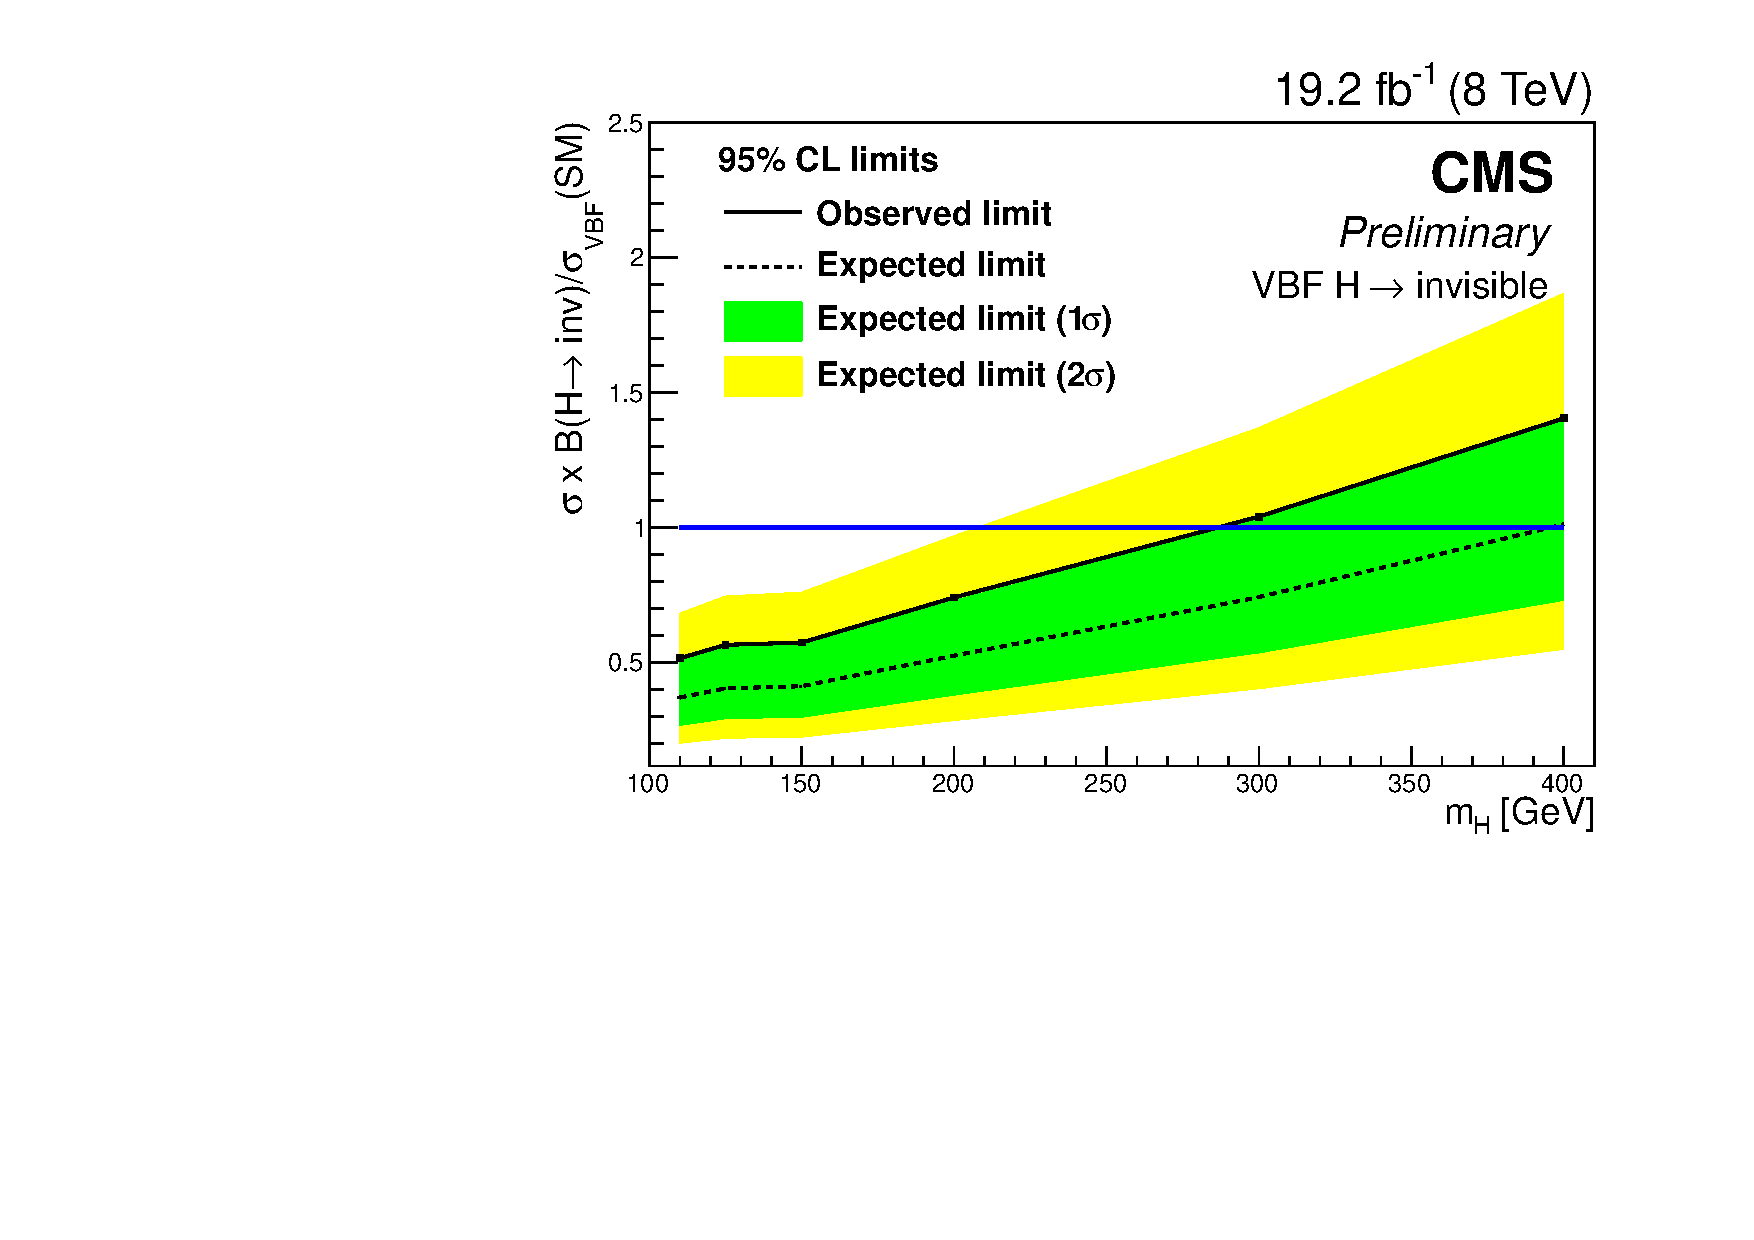
\includegraphics[width=\textwidth]{TalkPics/DM@LHC2016/Figure_007-a.pdf}
      \centering
      \scriptsize
      
      CMS-PAS-HIG-14-038
    \end{columns}
  \end{frame}

  \begin{frame}
    %??HIG-15-012
    \frametitle{Run 1 CMS direct searches - Combination}
    \vspace{-.2cm}
    \begin{block}{}
      \small
      \begin{itemize}
        \vspace{-.1cm}
      \item Combine by production mode as well as full combination
        \vspace{-.2cm}
      \item[-] ggH-tagged is monojet, VH-tagged is Z($\ell\ell$)H+Z($bb$)H+V(had)H, VBF-tagged is VBF
      \item Obs. (exp.) limit on $\mathcal{B}\left(H\rightarrow inv.\right)$ at $m_{H}=$125 GeV is 36 (30)\%
      \end{itemize}
    \end{block}
    \begin{columns}
      %??by category plot
      \column{.5\textwidth}
      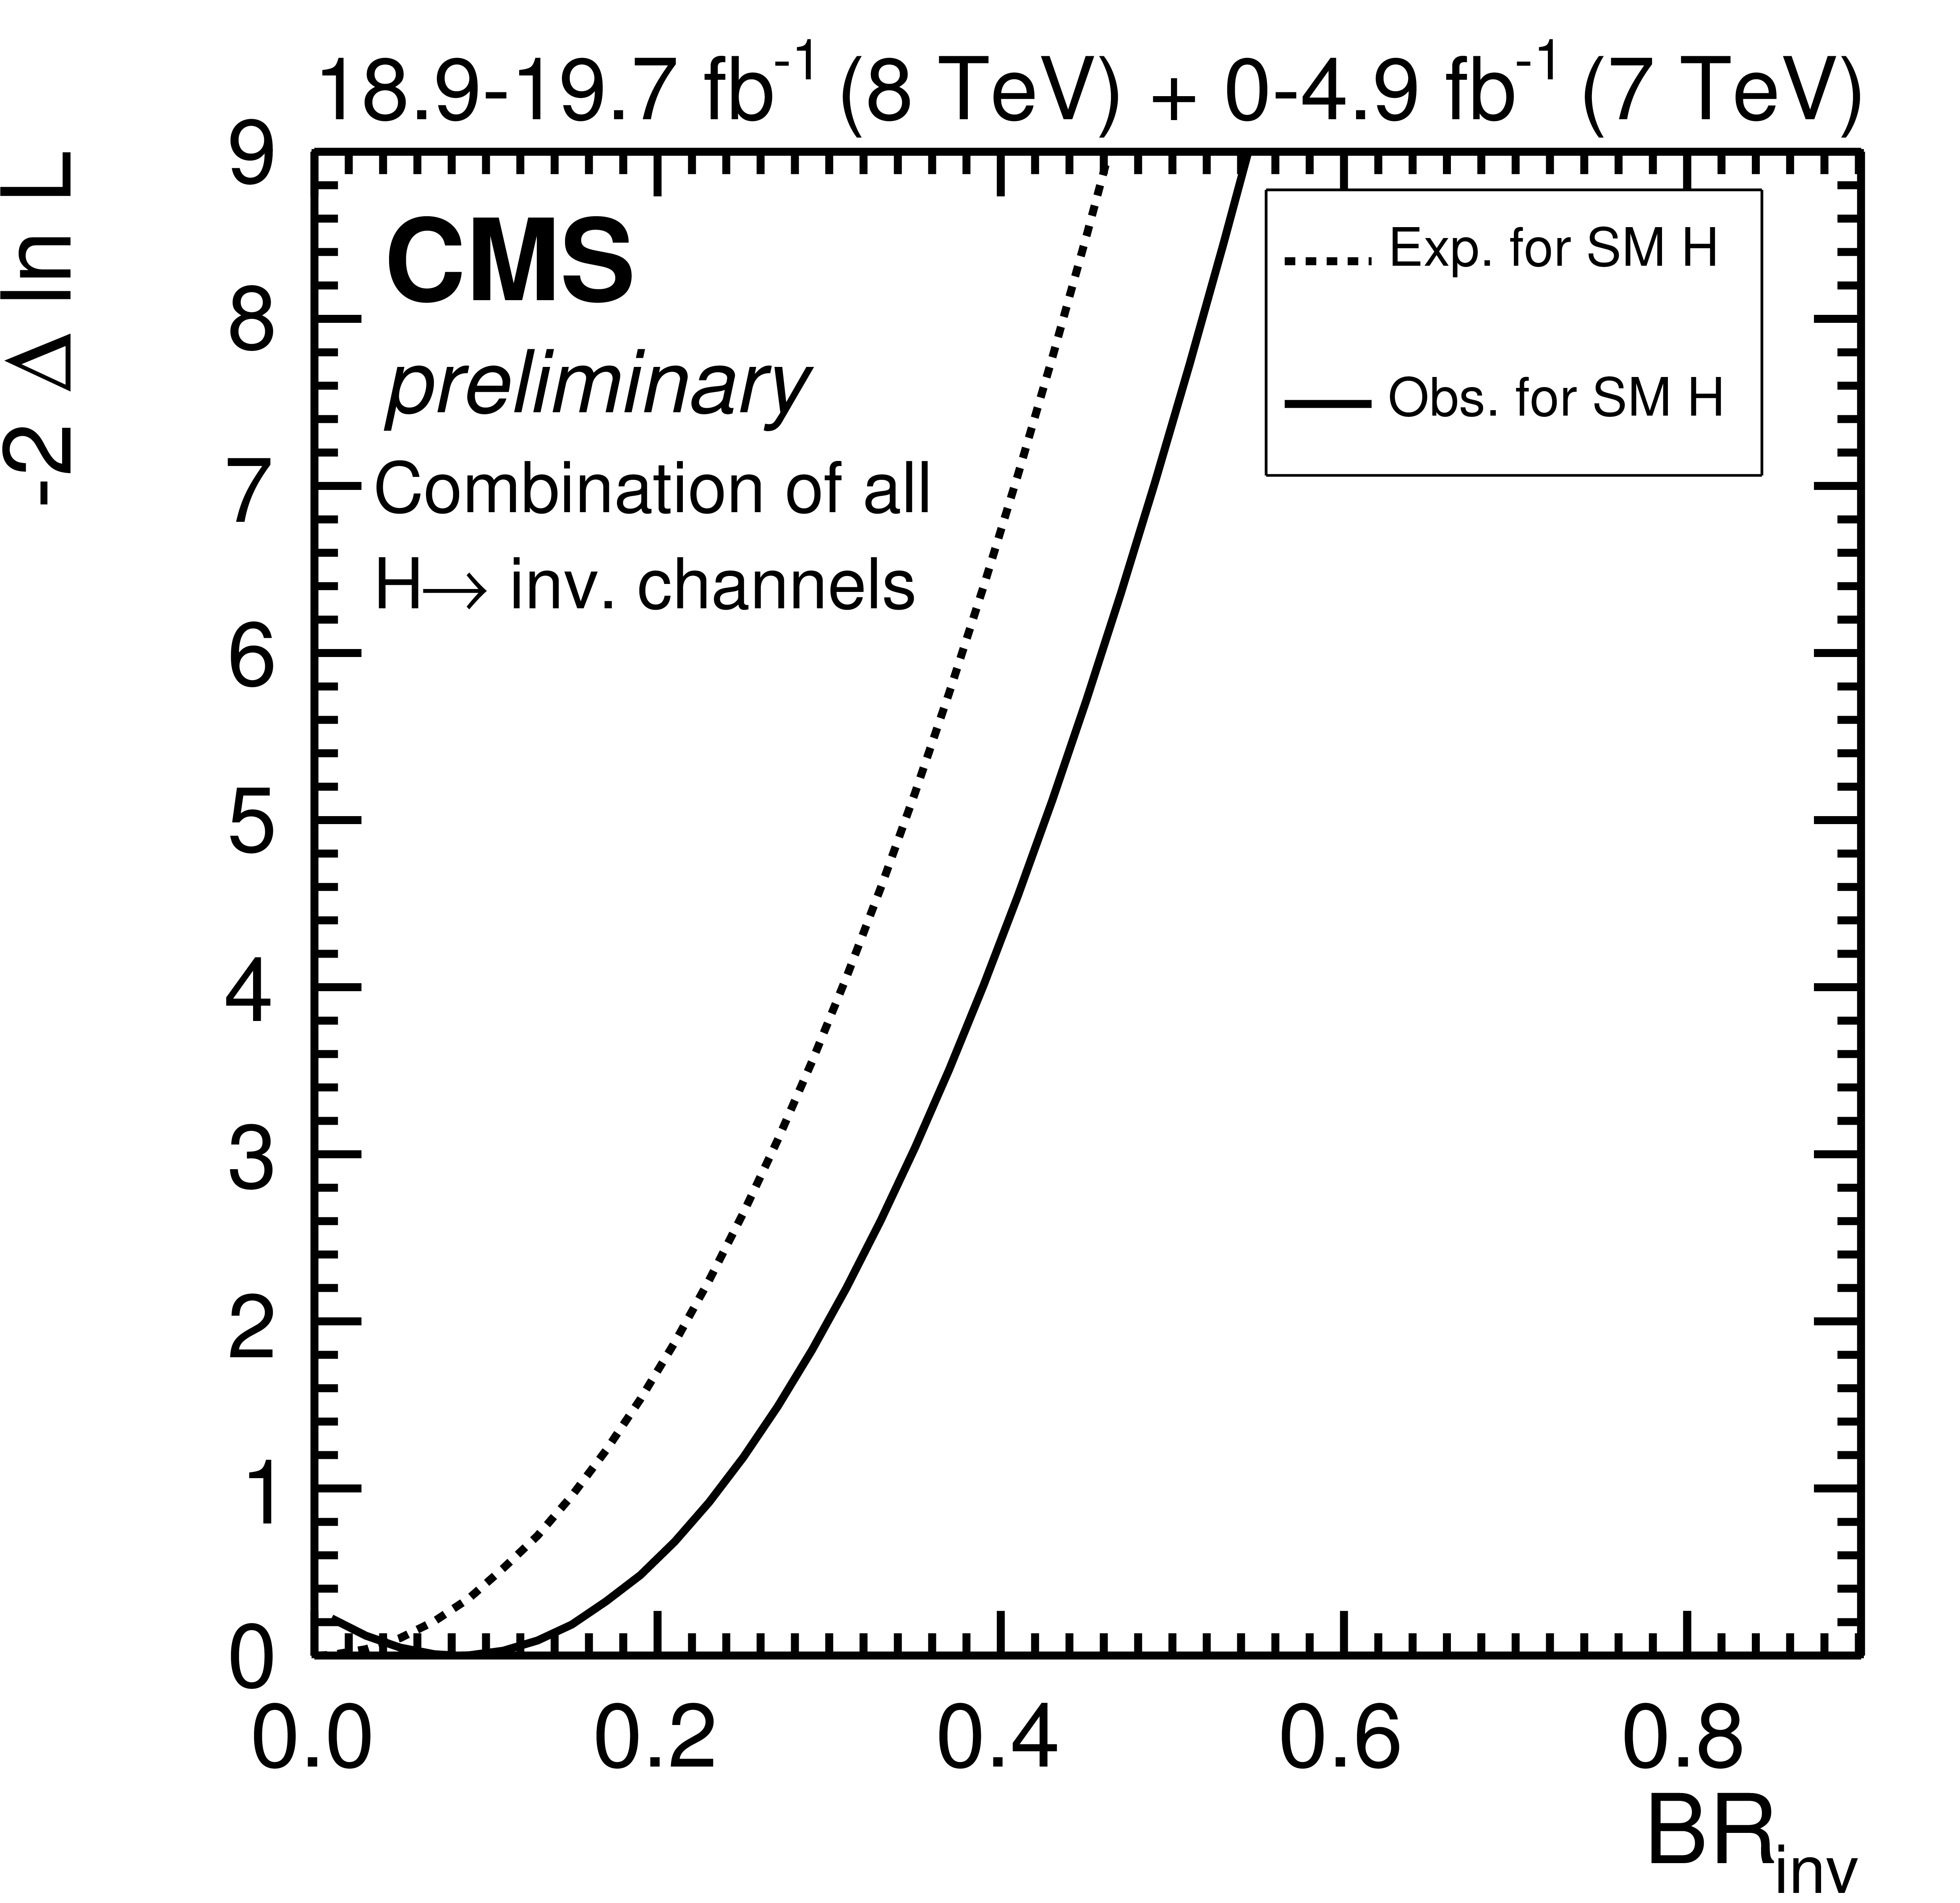
\includegraphics[width=.8\textwidth]{TalkPics/DM@LHC2016/CMS-PAS-HIG-15-012_Figure_002.png}
      \column{.5\textwidth}
      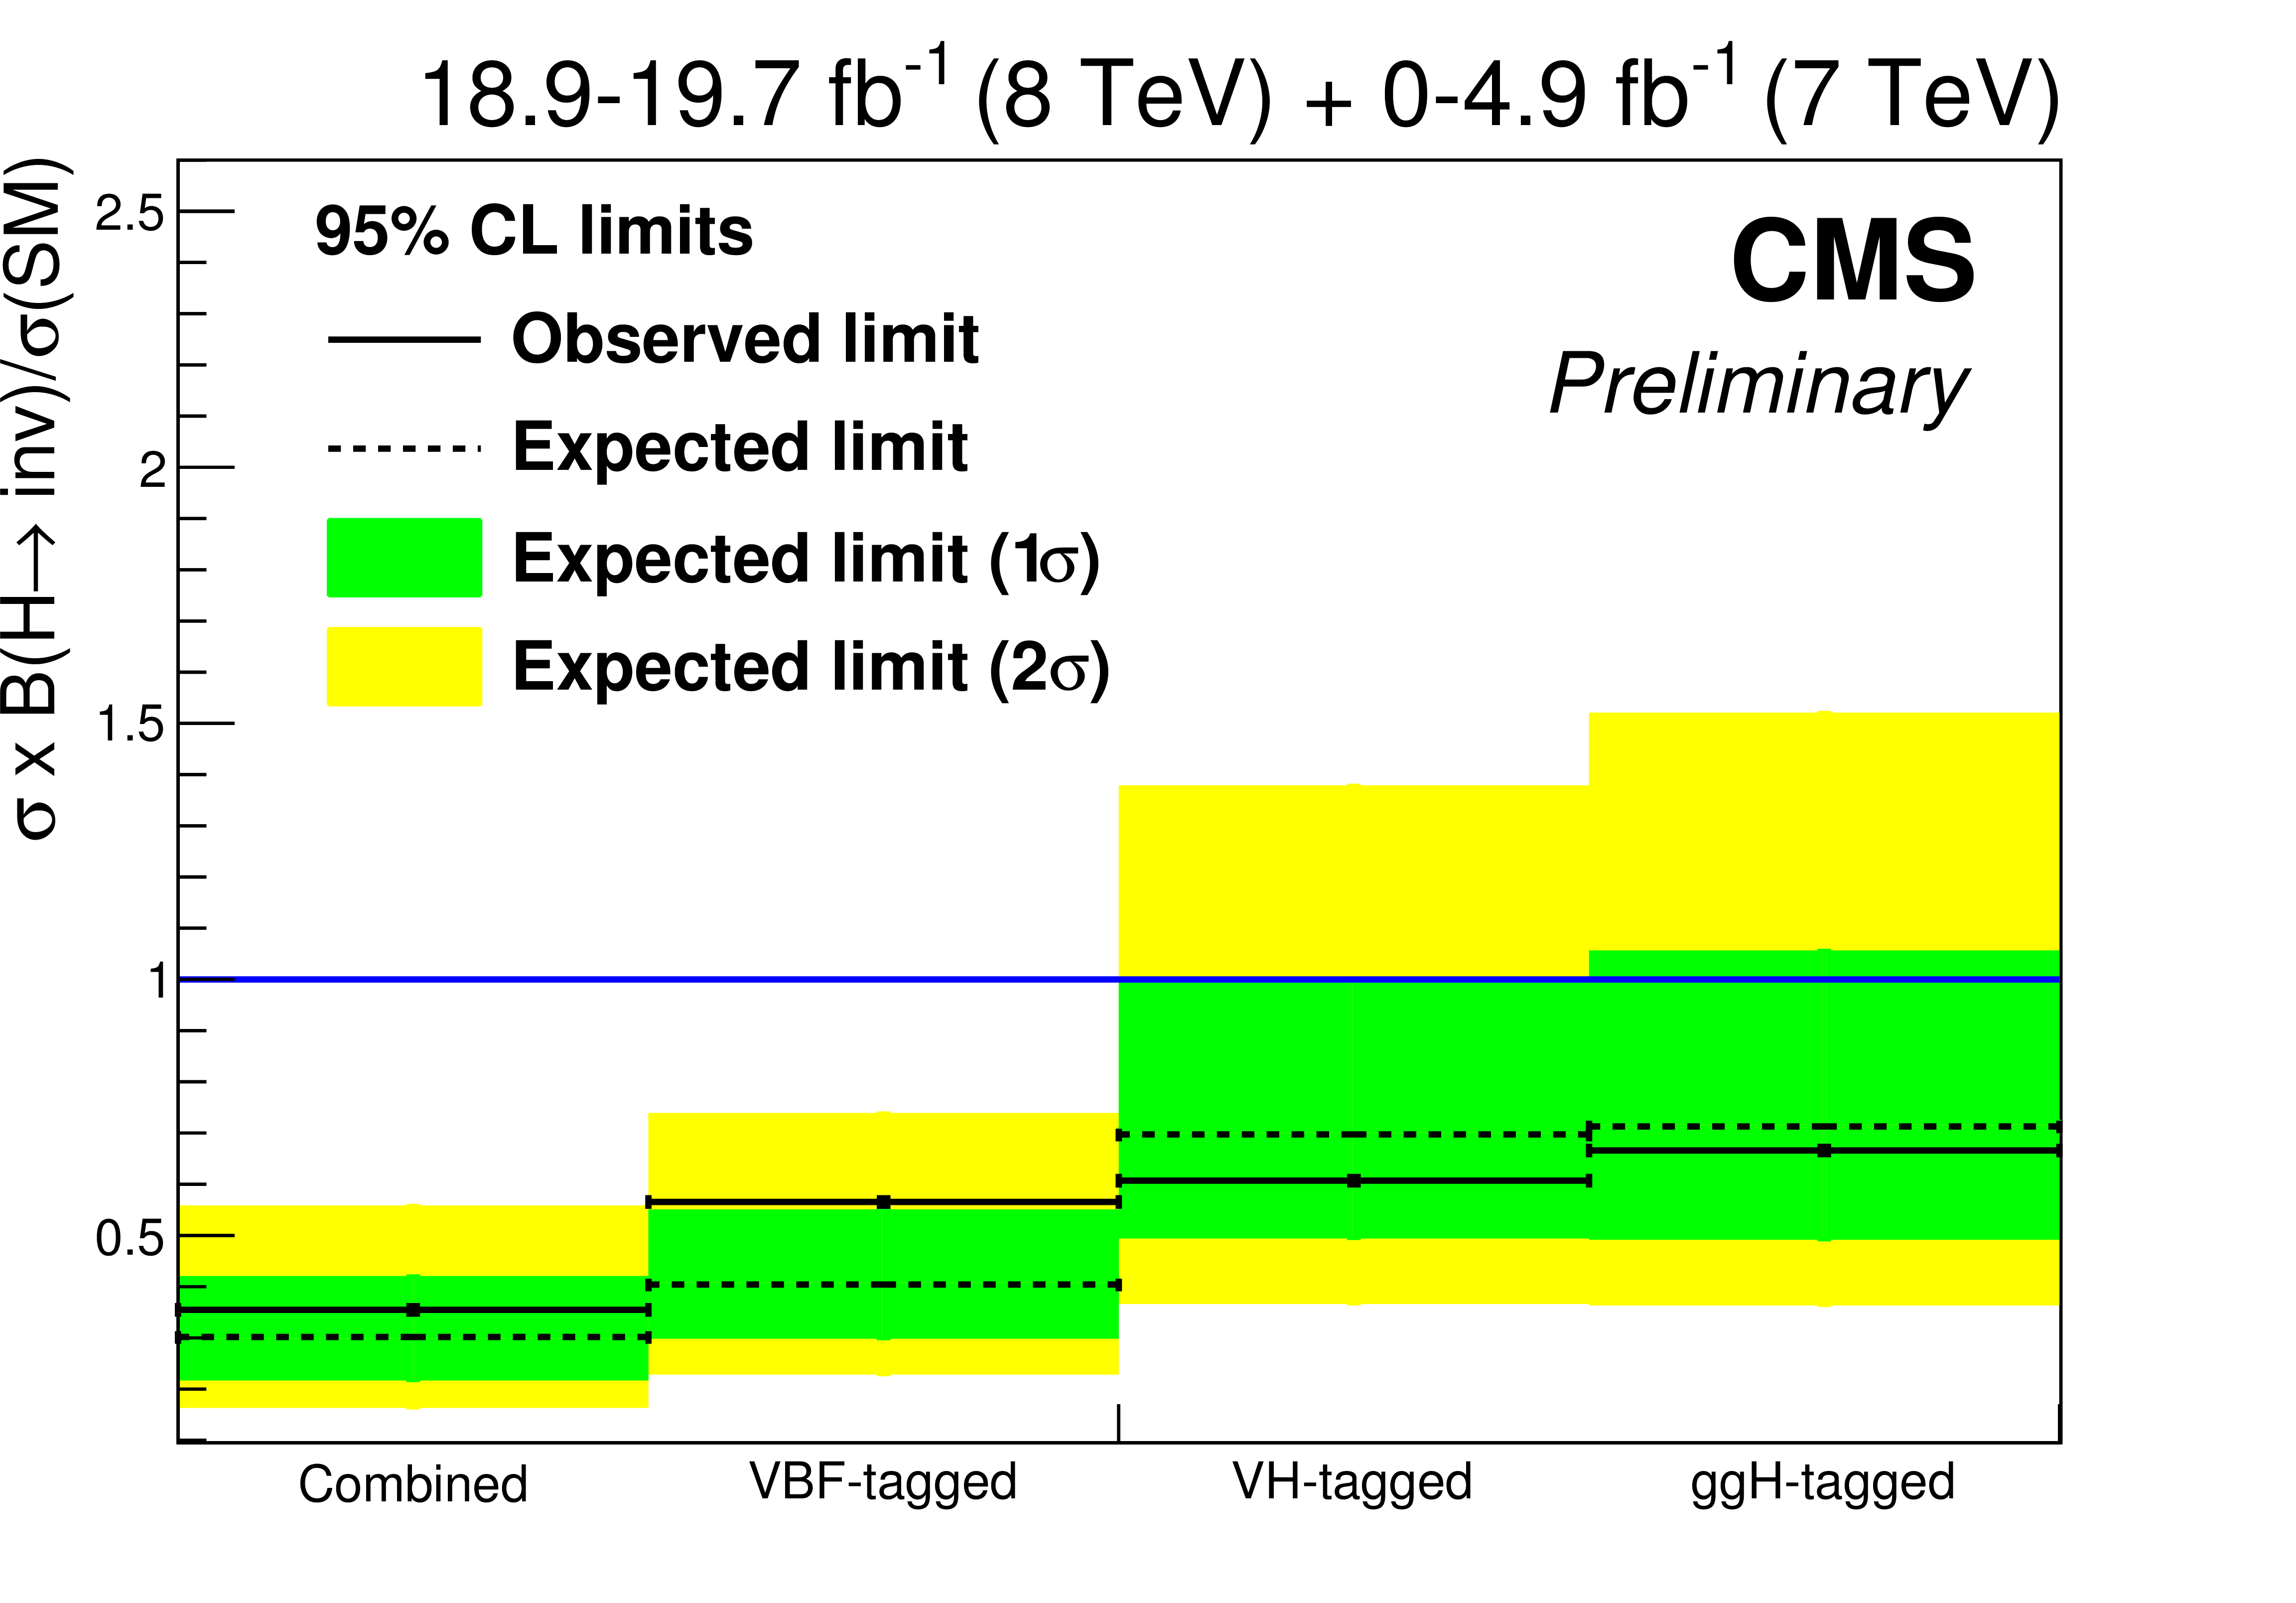
\includegraphics[width=.9\textwidth]{TalkPics/DM@LHC2016/CMS-PAS-HIG-15-012_Figure_003.png}
    \end{columns}
    \centering
    \scriptsize
    
    CMS-PAS-HIG-15-012
  \end{frame}

  %??CMS Run 2
  \begin{frame}
    %??HIG-16-008
    \frametitle{Run 2 CMS direct searches - ZH}
    %??fig 3c, mention move away from mass scans in BR
    \begin{columns}
      \column{.5\textwidth}
      \begin{block}{}
        \small
        \begin{itemize}
        \item Targets $Z\rightarrow\ell\ell$ final state
        \item 2D shape analysis with leading backgrounds estimated using MC
        \item Observed (expected) limit on $\mathcal{B}\left(H\rightarrow inv.\right)$ for $m_{H}=$125 GeV is 124 (124)\%
        \end{itemize}
      \end{block}
      \column{.5\textwidth}
      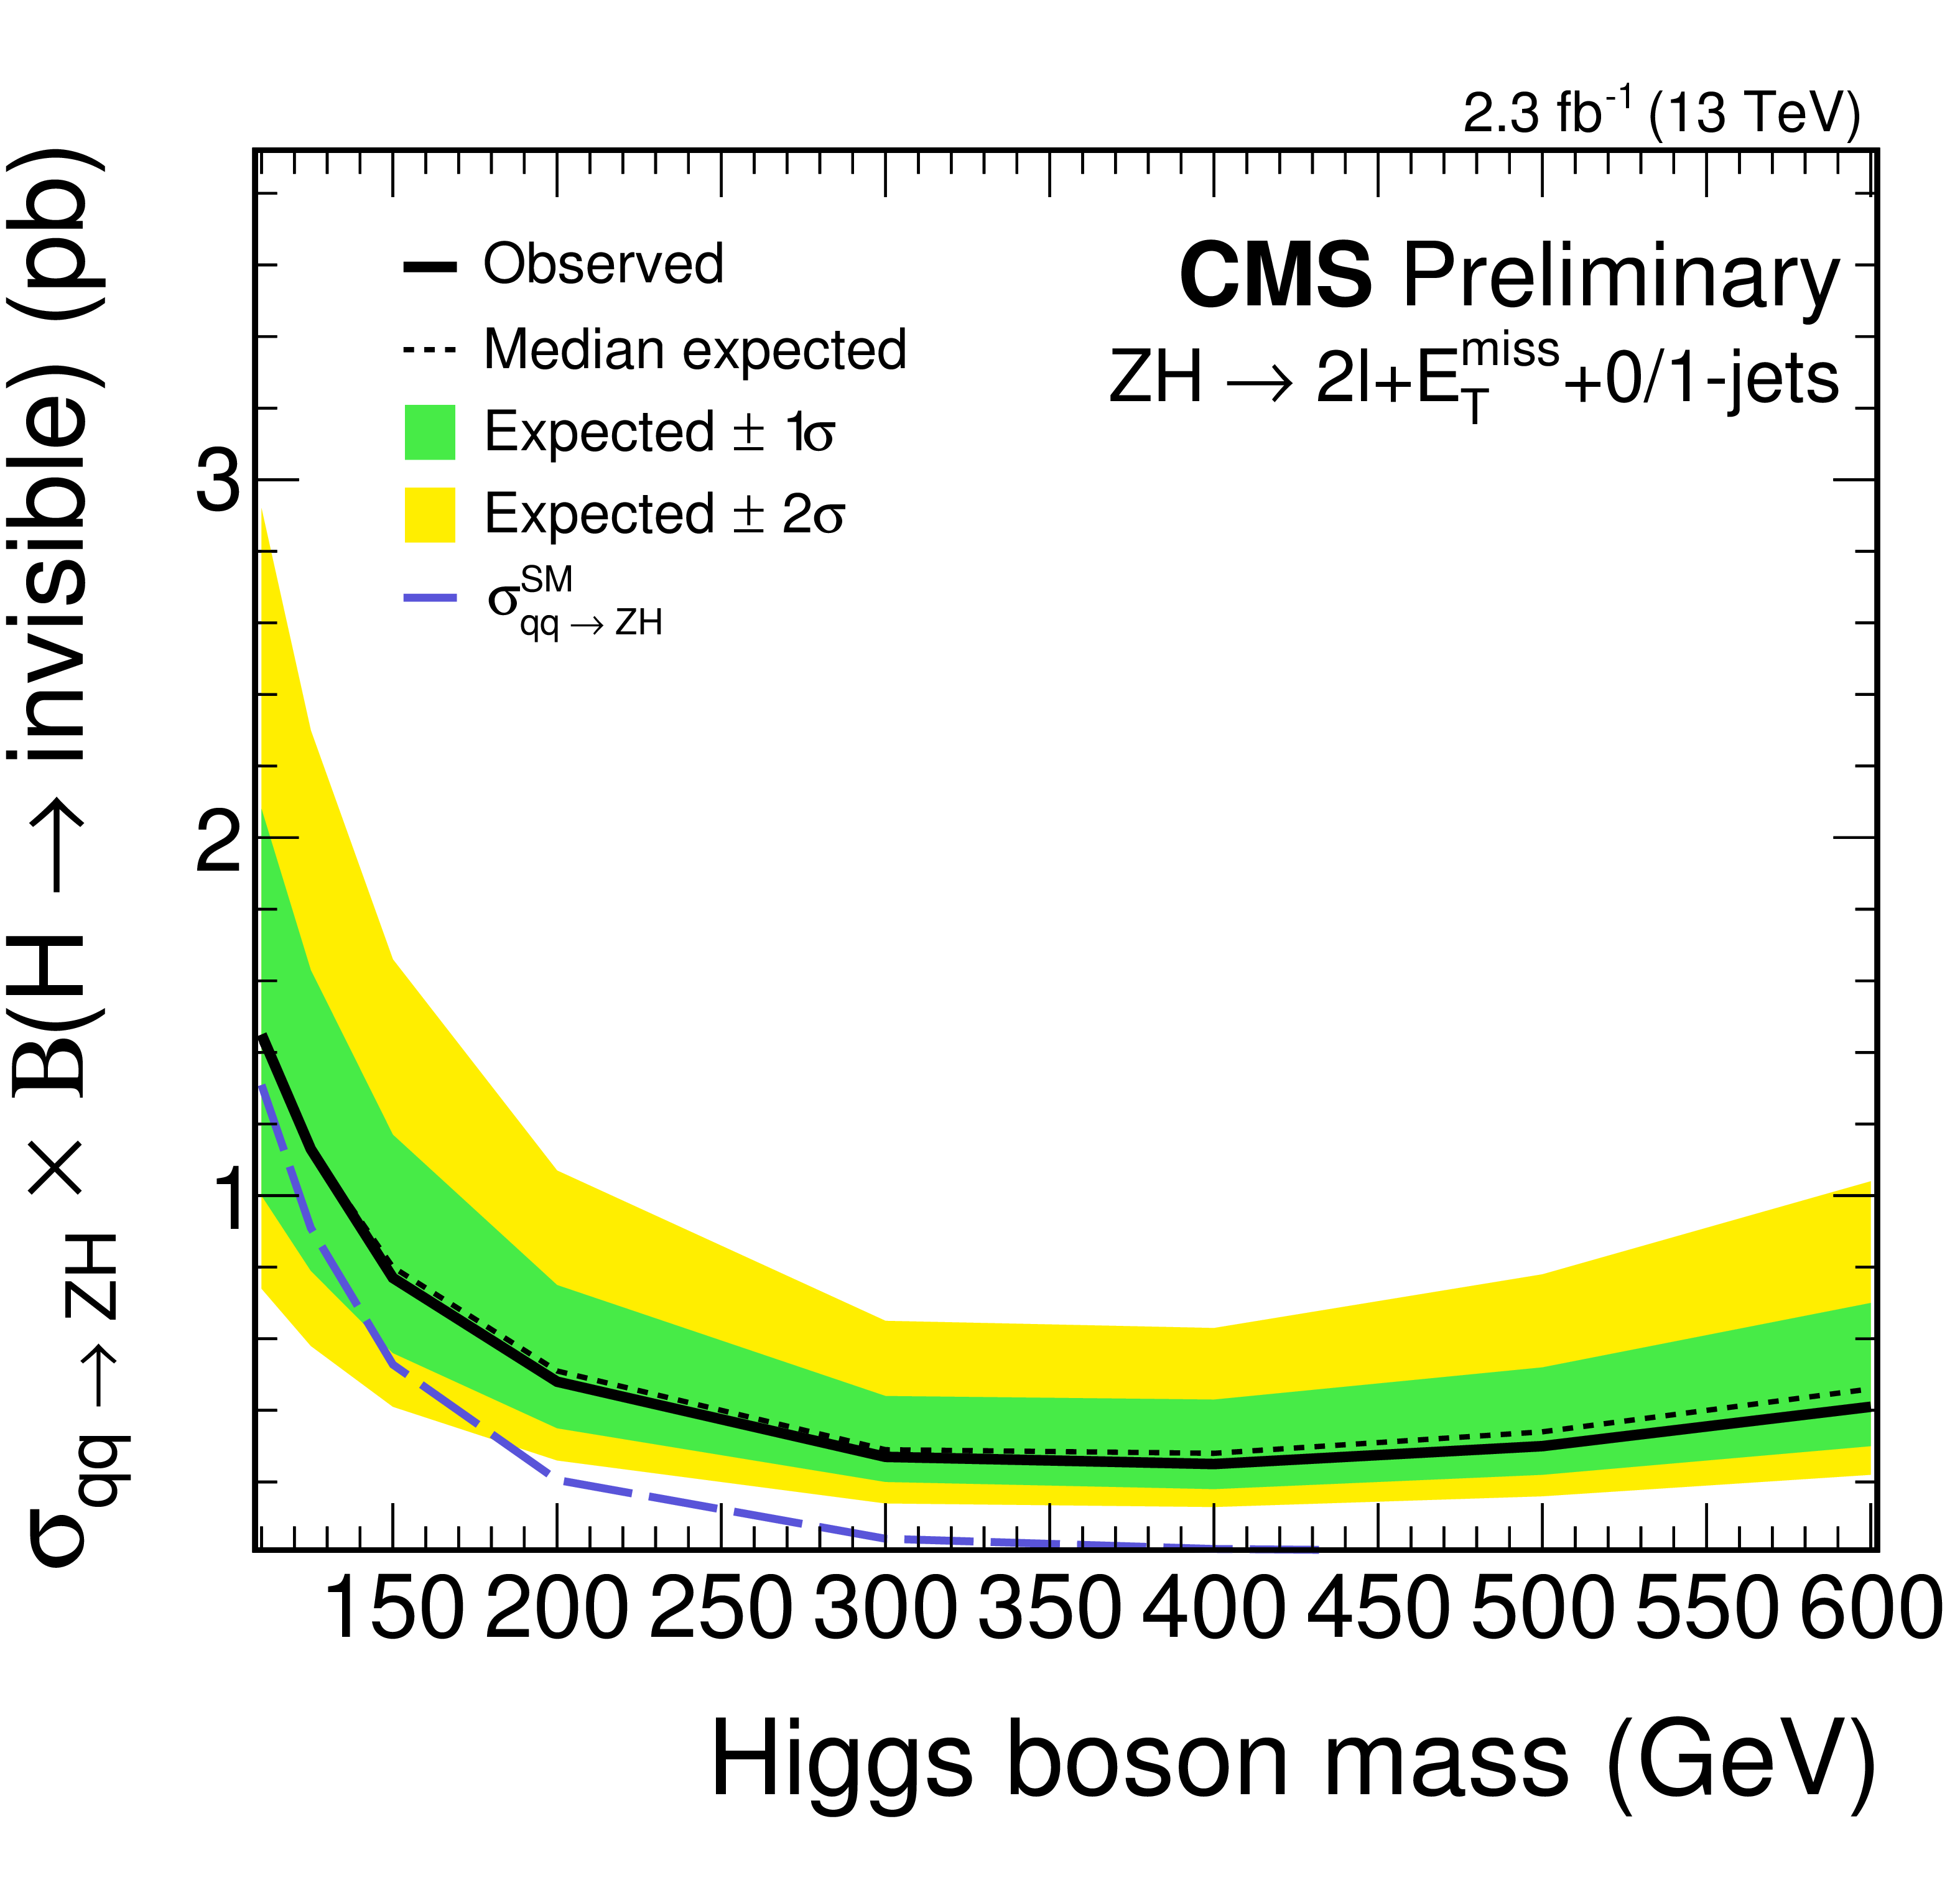
\includegraphics[width=\textwidth]{TalkPics/DM@LHC2016/CMS-PAS-HIG-16-008_Figure_003-c.png}
      \centering
      \scriptsize
      
      CMS-PAS-HIG-16-008
    \end{columns}
  \end{frame}

  \begin{frame}
    %??HIG-16-009
    \frametitle{Run 2 CMS direct searches - VBF}
    %??mass scan plot, WZ tying together
    \begin{columns}
      \column{.5\textwidth}
      \begin{block}{}
        \small
        \begin{itemize}
        \item Dedicated trigger used again
        \item Counting experiment with data driven background estimation
        \item V+jets backgrounds all taken to have same normalisation
        \item Observed (expected) limit on $\mathcal{B}\left(H\rightarrow inv.\right)$ for $m_{H}=$125 GeV is 69 (62)\% 
        \end{itemize}
      \end{block}
      \column{.5\textwidth}
      %??mass scan
      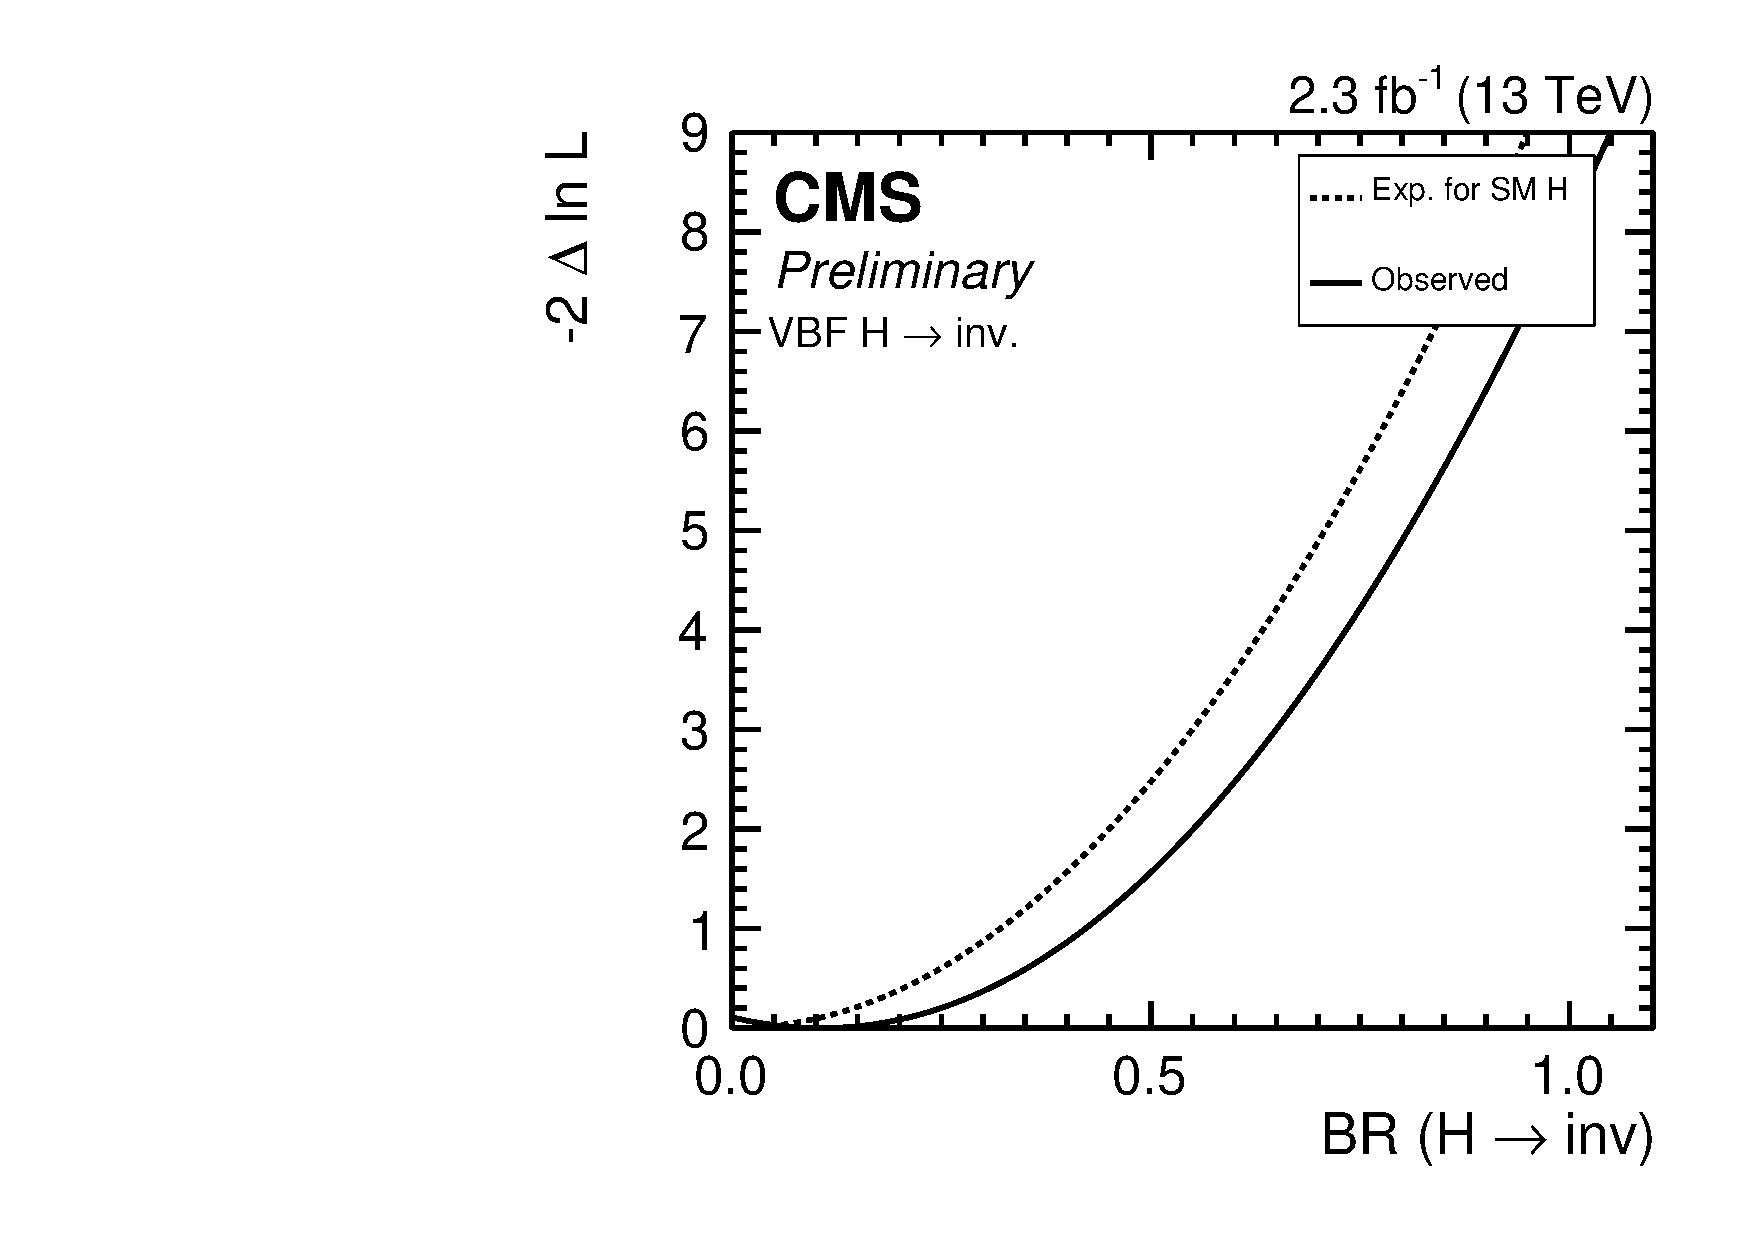
\includegraphics[width=\textwidth]{TalkPics/DM@LHC2016/brlhscan.pdf}
      \centering
      \scriptsize
      
      CMS-PAS-HIG-16-009
    \end{columns}
  \end{frame}
  
  %??HIG-16-009 Combination CMS Run 1 + Run 2
  \begin{frame}
    \frametitle{Run 2 CMS direct searches - Combination}
    %??explain contributing analyses
    %??13 TeV only and 8 TeV+13 TeV category plot
    \begin{block}{}
      \begin{itemize}
      \item First CMS analysis combining 8 and 13 TeV results
      \item Limit calculated both by production mode and overall
      \item Combined observed (expected) limit on $\mathcal{B}\left(H\rightarrow inv.\right)$ for $m_{H}=$125 GeV is 32 (26)\% %??
      \end{itemize}
      
    \end{block}
    \begin{columns}
      \column{.5\textwidth}
      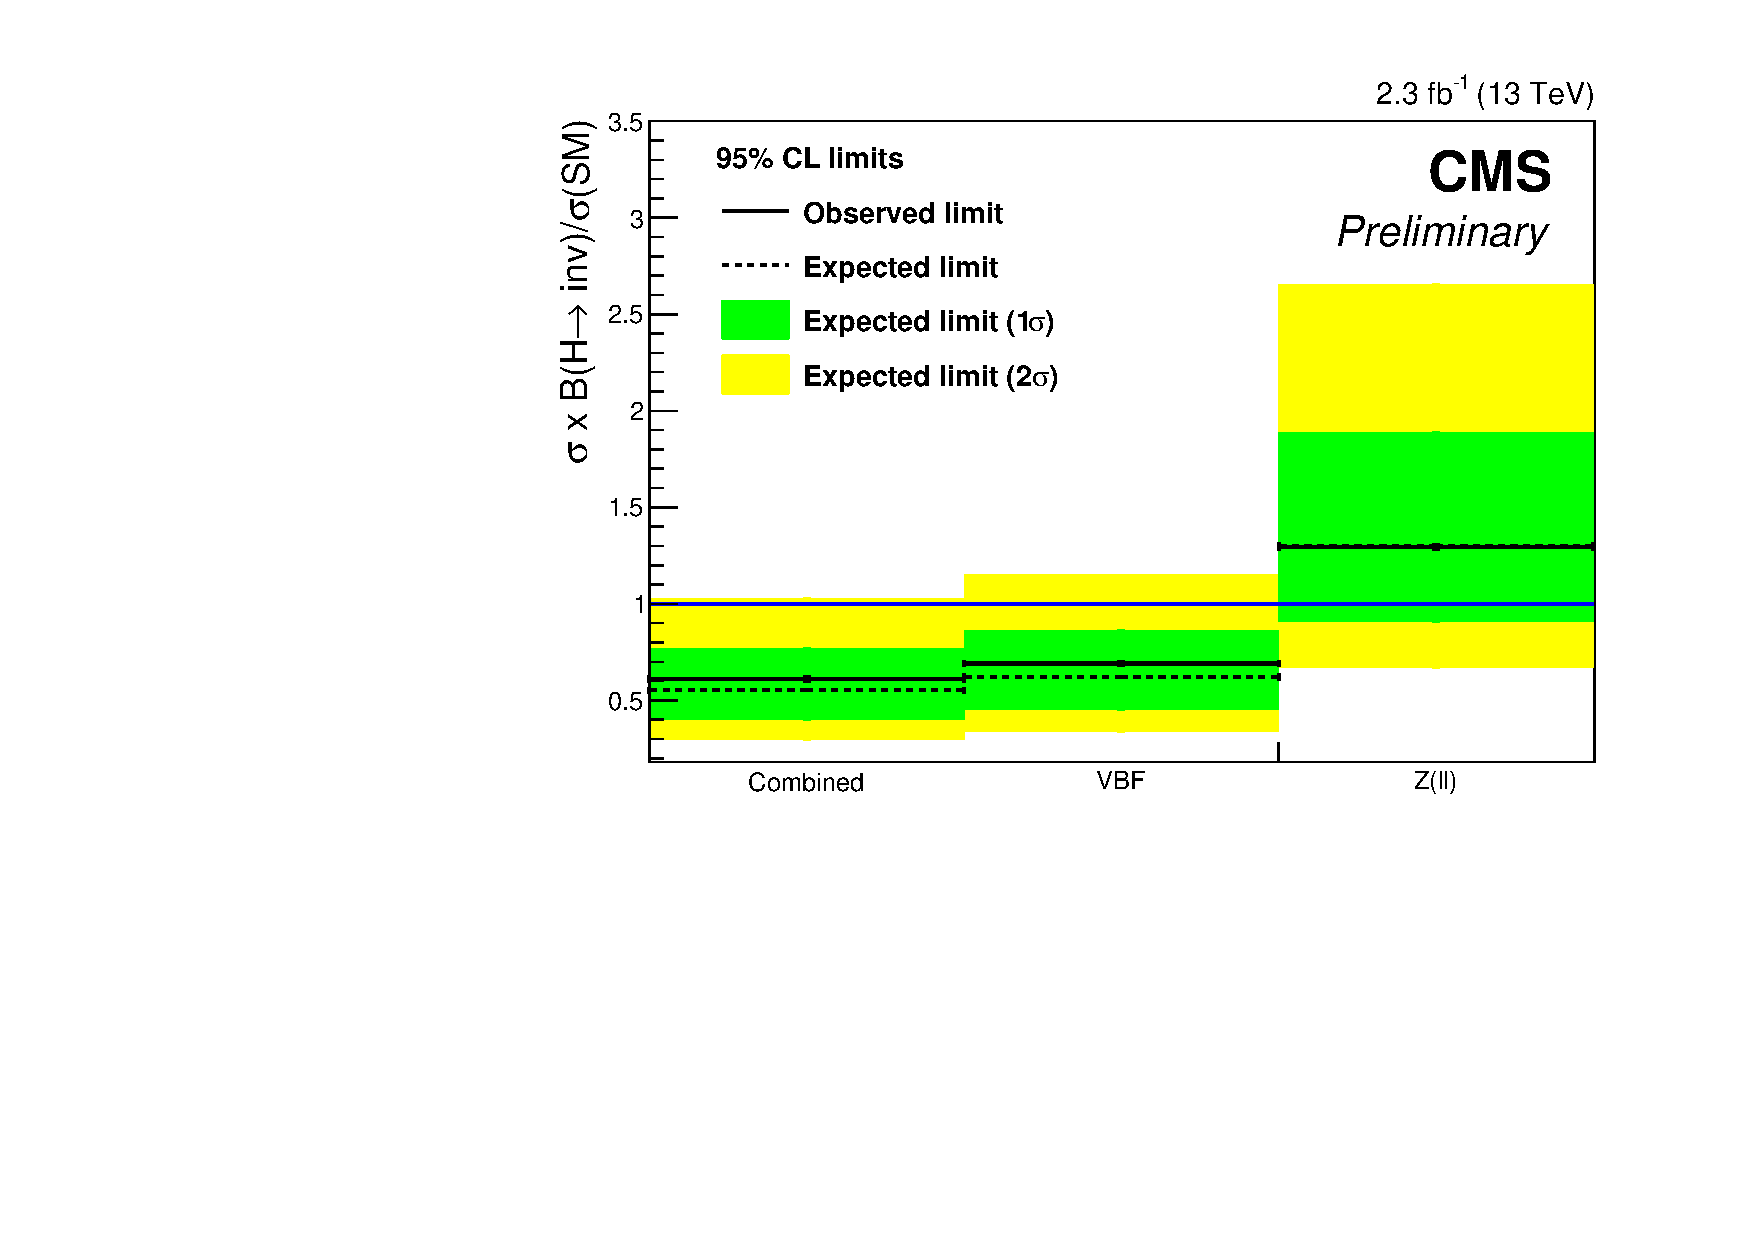
\includegraphics[width=\textwidth]{TalkPics/DM@LHC2016/channellimit13_withoutMono.pdf}
      \column{.5\textwidth}
      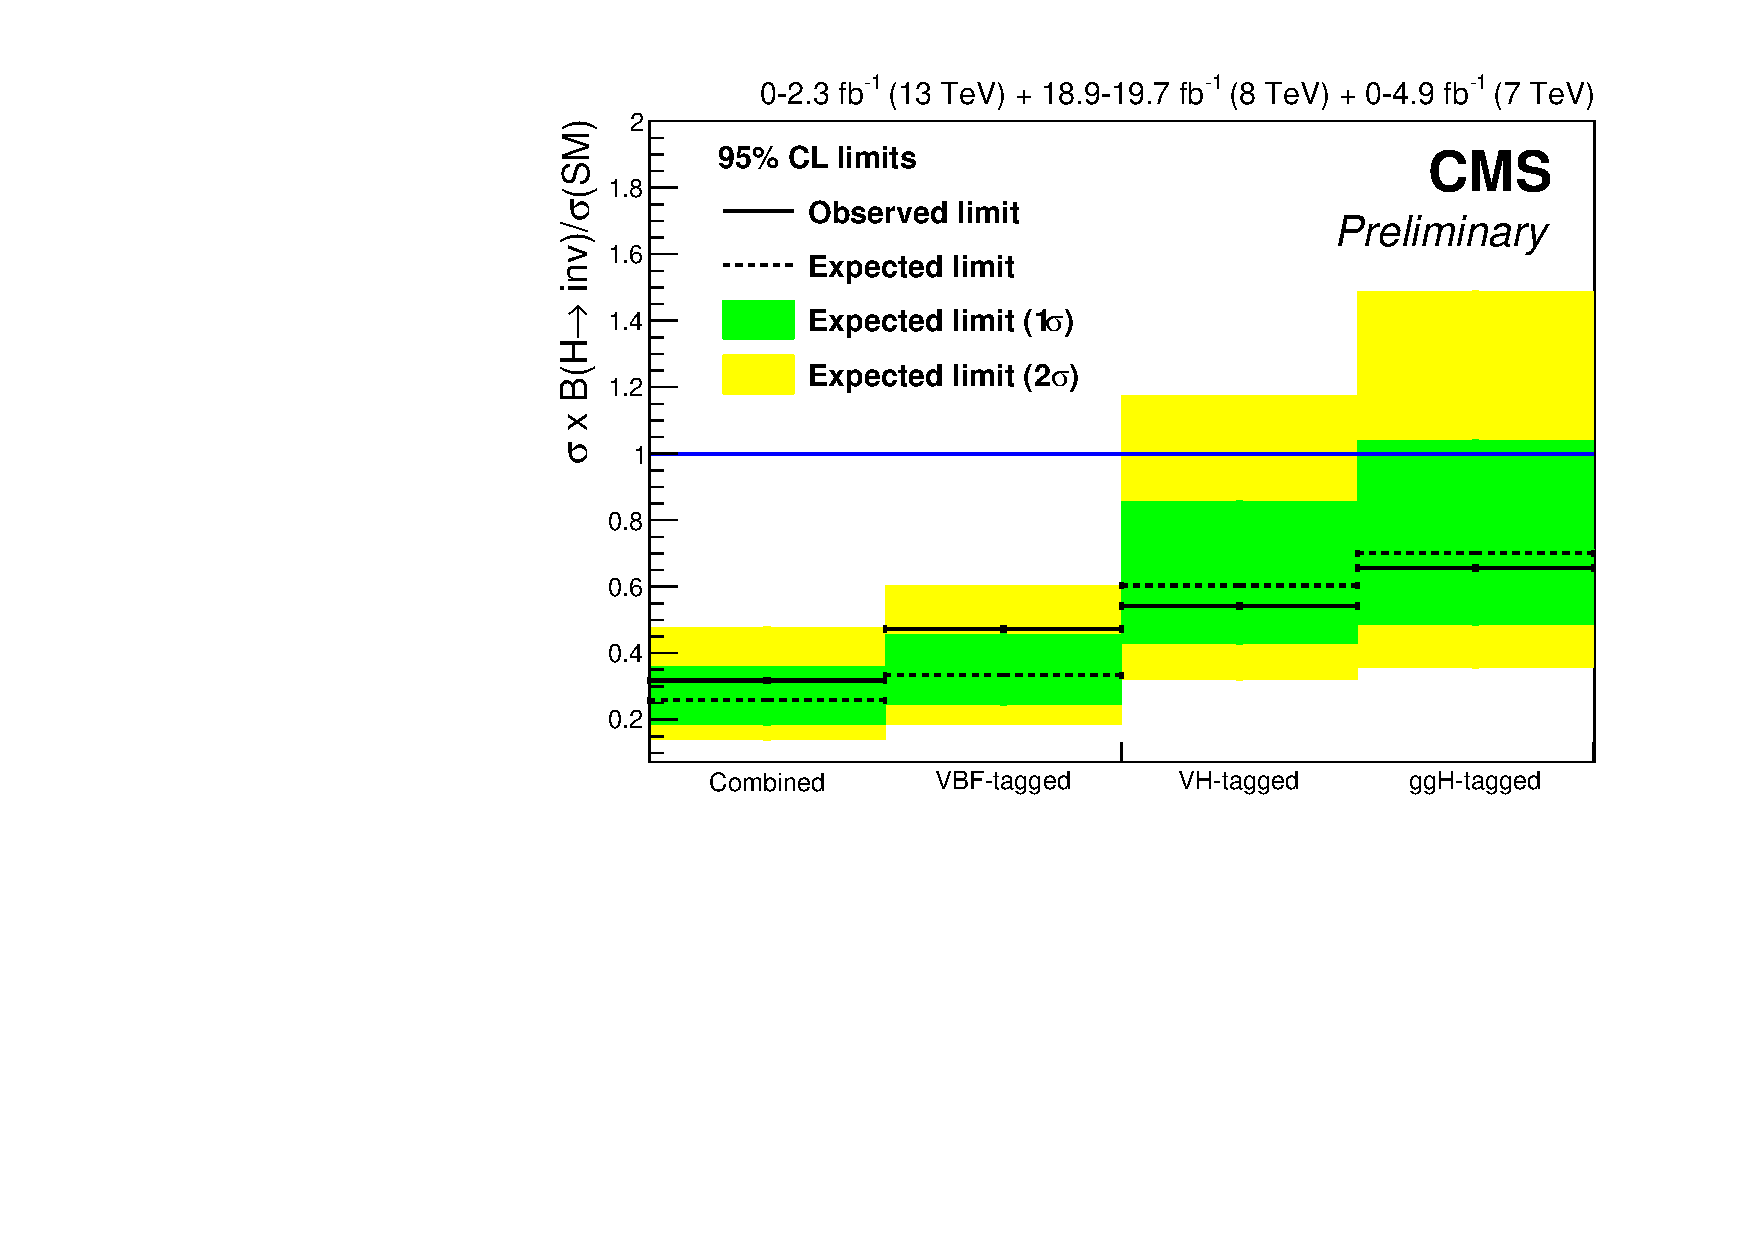
\includegraphics[width=\textwidth]{TalkPics/DM@LHC2016/channellimit.pdf}
    \end{columns}
    \centering
    \scriptsize
    
    CMS-PAS-HIG-16-009
  \end{frame}

  

  %??DM pheno paper
  \begin{frame}
    \frametitle{Projections}
    \begin{columns}
      \column{.5\textwidth}
      \begin{block}{}
        \small
        \begin{itemize}
        \item CMS VBF analysis projected to increased luminosity at 13 TeV
        \item If systematics scale as $\sqrt{\mathcal{L}}$ can exclude $\mathcal{B}\left(H\rightarrow inv.\right)=5\%$ with full LHC dataset
        \end{itemize}
      \end{block}
      \column{.5\textwidth}
      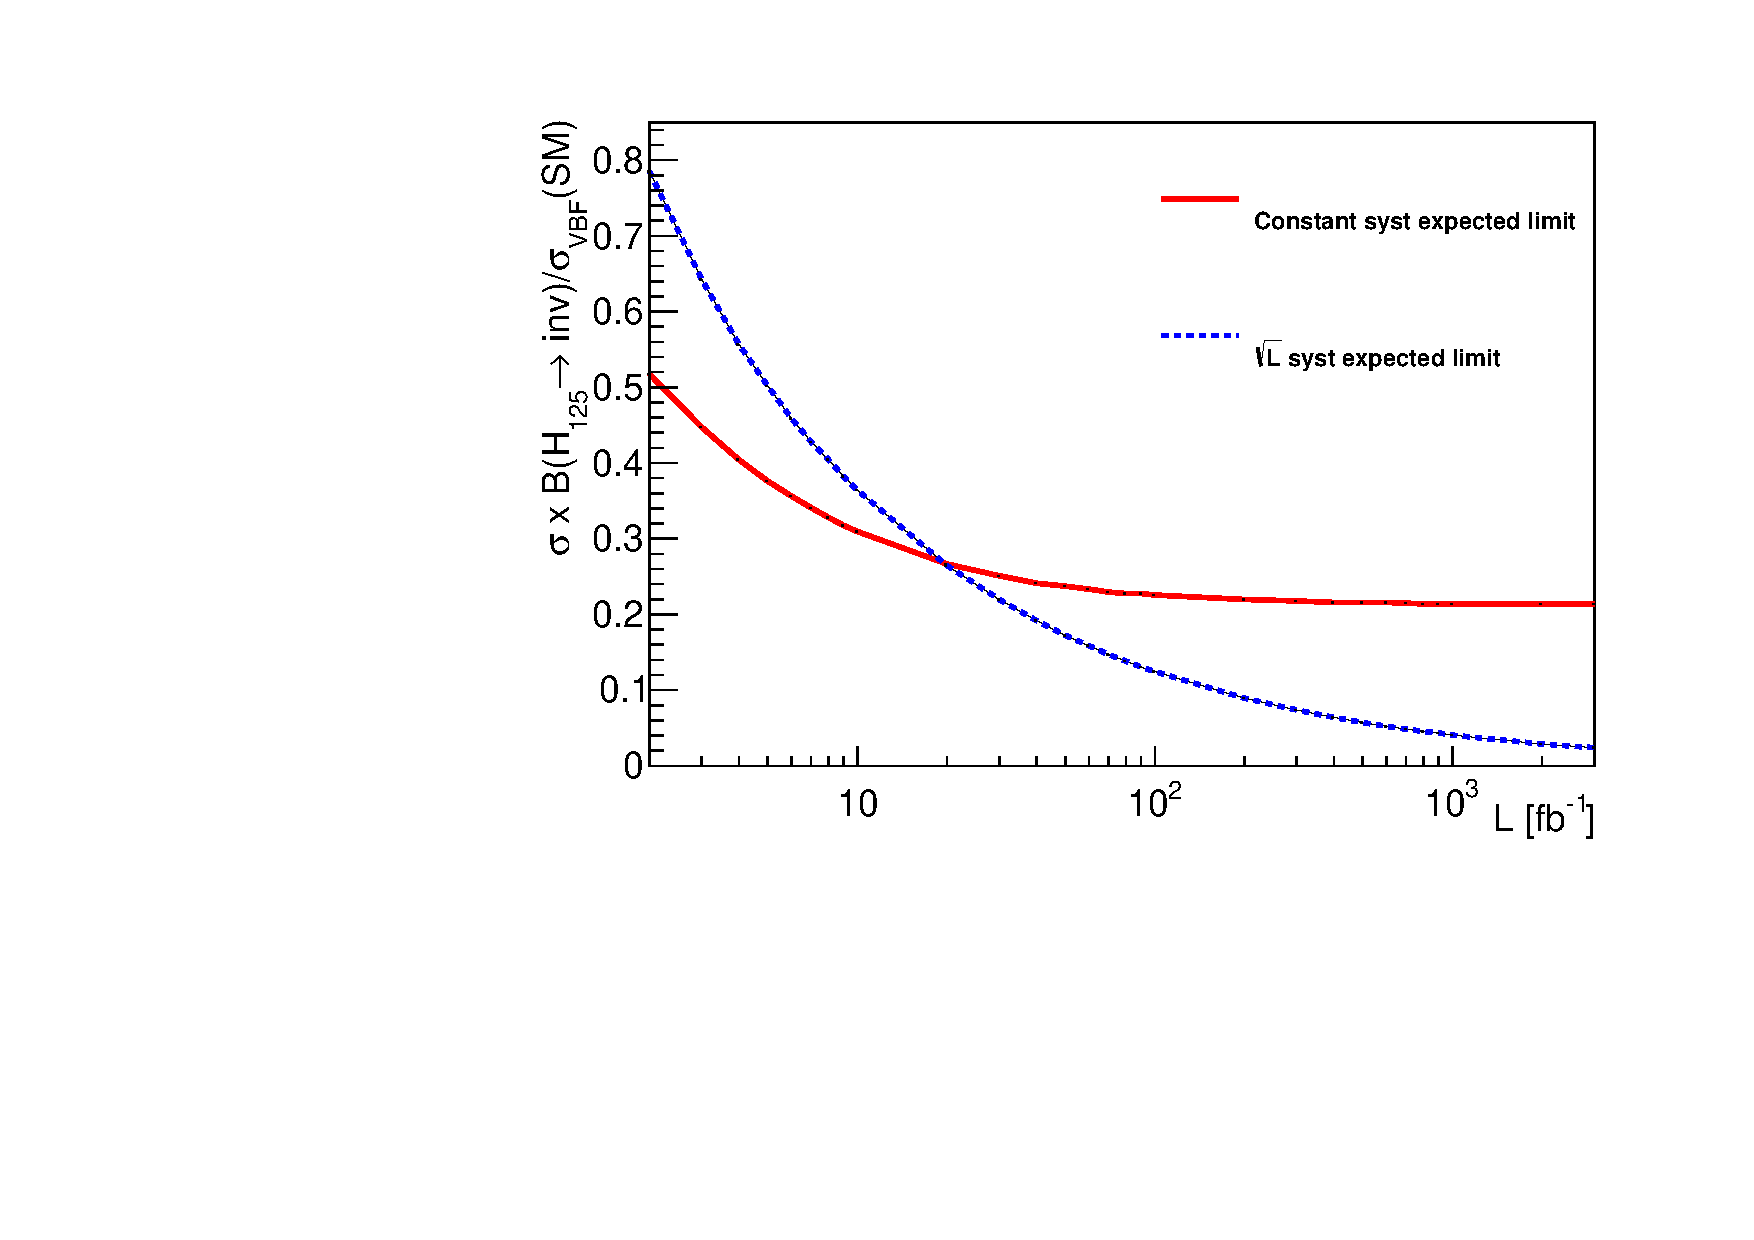
\includegraphics[width=\textwidth]{TalkPics/DM@LHC2016/phenoprojectedvbflimit.pdf}
      \centering
      \scriptsize

      arXiv:1603.07739
    \end{columns}
  \end{frame}

  \begin{frame}
    \frametitle{Dark matter interpretations - Run 1 results}
    %??ATLAS DM plot and arxiv EFT plane plot
    \begin{columns}
      \column{.5\textwidth}
      \begin{block}{}
        \small
        \begin{itemize}
        \item Several models for interpreting invisible Higgs limits
          \vspace{-.1cm}
        \item ``Higgs portal'' has been quite commonly used
          \vspace{-.2cm}
        \item[-] Assume 125 GeV Higgs acts as mediator between visible and dark matter sectors
          \vspace{-.2cm}
        \item[-] Assume scalar, fermion or vector dark matter
          \vspace{-.1cm}
        \item Scalar dark matter would mix with Higgs boson
          \vspace{-.2cm}
        \item[-] mixing angle must be small
          \vspace{-.1cm}
        \item Vector dark matter width goes to infinity as mass decreases
        \end{itemize}
      \end{block}      

      \column{.5\textwidth}

      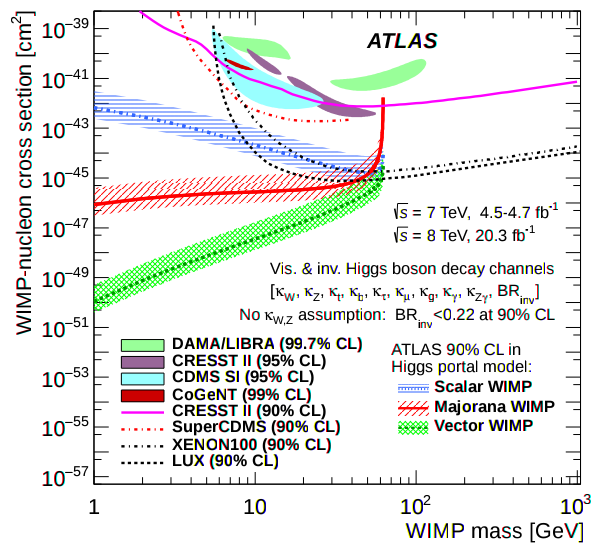
\includegraphics[width=\textwidth]{TalkPics/DM@LHC2016/ATLASdmlimit.png}
      \centering
      \scriptsize

      JHEP11(2015)206      
    
    \end{columns}
  \end{frame}

  \begin{frame}
    \frametitle{Dark matter interpretations - Projections}
    \begin{block}{}
      \small
      \begin{itemize}
      \item Models with electroweak couplings studied: favours VBF channel
      \item VBF topology allows looser $E_{T}^{miss}$ selection making EFTs valid
      \item Also investigate simplified models with scalar/pseudoscalar mediator
      \item Projections of CMS VBF channel sensitivity at several luminosities
      \end{itemize}
    \end{block}
    \begin{columns}
      \column{.5\textwidth}
      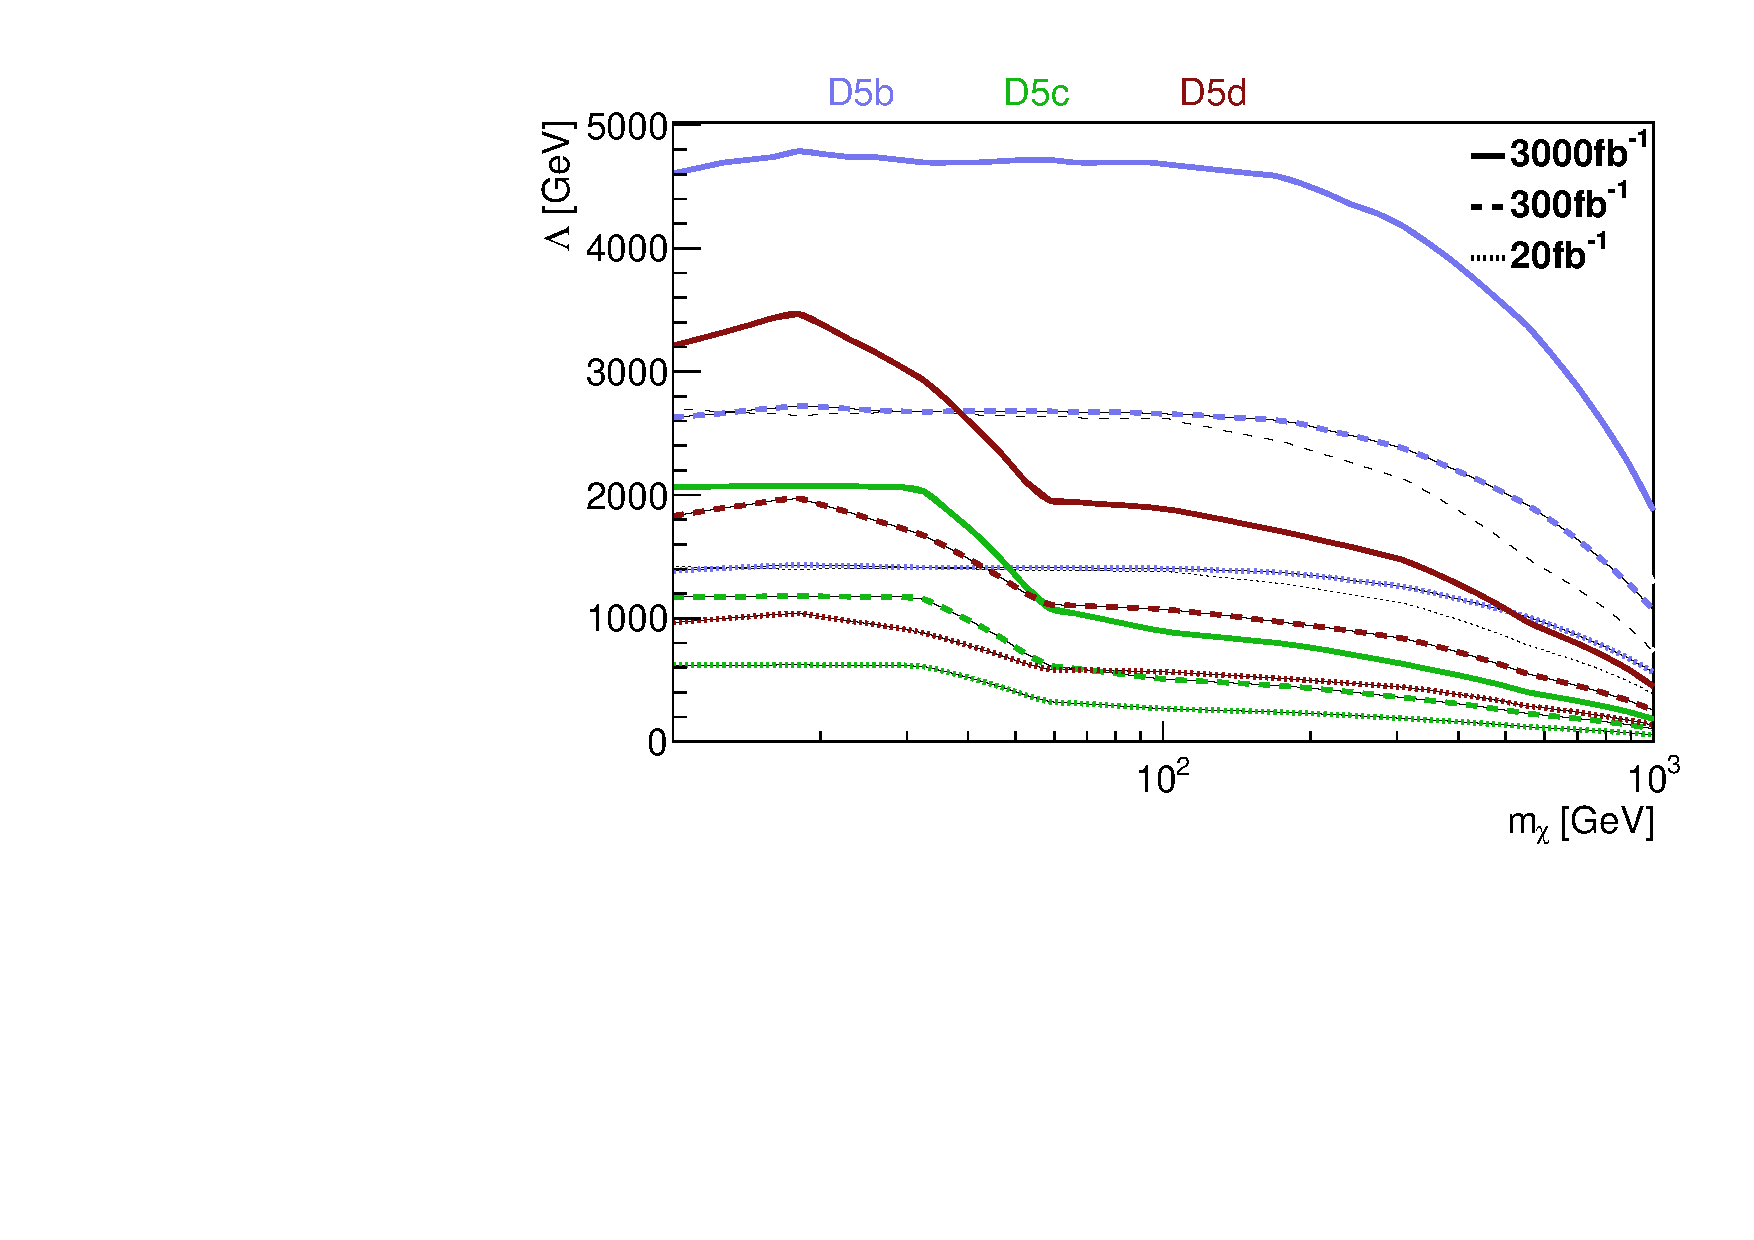
\includegraphics[width=\textwidth]{TalkPics/DM@LHC2016/D5_multilumi.pdf}
      \column{.5\textwidth}
      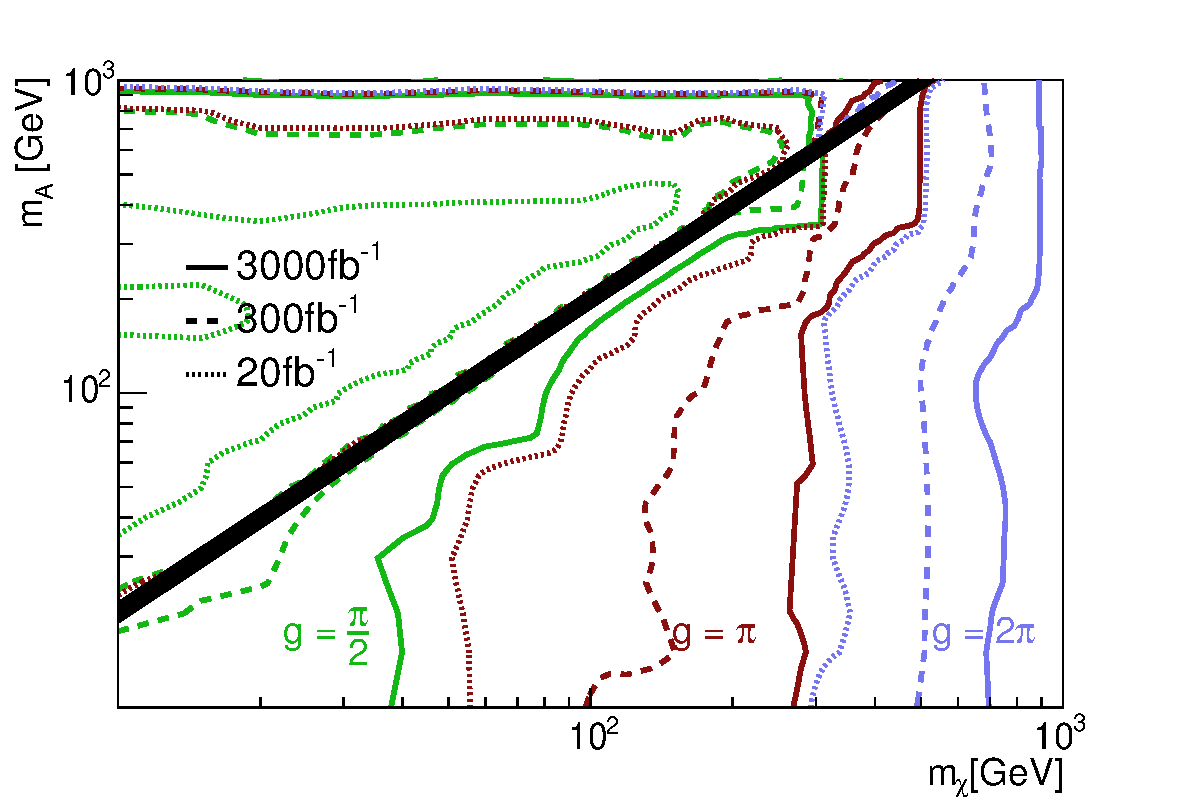
\includegraphics[width=\textwidth]{TalkPics/DM@LHC2016/Aplane.pdf}      
    \end{columns}
      \centering
      \scriptsize

      arXiv:1603.07739
  \end{frame}

  \begin{frame}
    \frametitle{Summary}
    \label{lastframe}
    \begin{block}{}
      \begin{itemize}
      \item Both collaborations are sensitive to $\mathcal{B}\left(H\rightarrow inv.\right)\sim 25\%$ with current datasets
      \item[-] Current 95\% CL upper observed (expected) limits from direct searches are CMS: 32 (26)\%, ATLAS: 25 (27) \%
      \item[-] Combinations of channels allow sensitivity to be greatly improved
      \item Projected limit on $\mathcal{B}\left(H\rightarrow inv.\right)\sim$10-20\% from VBF alone by the end of LHC Run 2 and 5\% by end of LHC running
      \end{itemize}
    \end{block}
  \end{frame}


  
\end{fmffile}
\end{document}

